\chapter{同伦类型论}
\label{cha:basics}

同伦类型论的核心新思想是：类型可以被看作同伦论中的空间，
或范畴论中的高维群胚。

\index{classical!homotopy theory|(}
\index{higher category theory|(}
我们先简要概述同伦论与高维范畴论之间的联系。
在经典同伦论中，空间 $X$ 是一个带拓扑结构的点集，
\indexsee{space!topological}{topological space}
\index{topological!space}
而点 $x$ 与 $y$ 之间的一条路径由连续映射
$p : [0,1] \to X$ 表示，其中 $p(0) = x$ 且 $p(1) = y$。
\index{path!topological}
\index{topological!path}
这个函数可以理解为：在每一个“时刻”都给出 $X$ 中的一个点。对许多目的而言，路径的严格相等
（即按点相等的函数）是过细的概念。例如，
可以定义路径拼接运算（若 $p$ 是从
$x$ 到 $y$ 的路径，$q$ 是从 $y$ 到 $z$ 的路径，则拼接 $p
\ct q$ 是从 $x$ 到 $z$ 的路径）以及逆路径（$\opp p$ 是从
$y$ 到 $x$ 的路径）。然而，这些运算之间存在一些自然方程，在严格相等下并不成立：例如，路径
$p \ct \opp p$（随时间从 $0$ 到 $1$，先从 $x$ 走到 $y$，再沿原路返回）并不与
恒等路径（在所有时刻都停留在 $x$）严格相等。

解决办法是考虑一种更粗糙的路径相等概念，称为
\emph{同伦}。
\index{homotopy!topological}
在一对连续映射 $f :
X_1 \to X_2$ 与 $g : X_1\to X_2$ 之间，一个同伦是连续映射 $H : X_1
\times [0, 1] \to X_2$，满足 $H(x, 0) = f (x)$ 且 $H(x, 1) =
g(x)$。在路径 $p$ 与 $q$（从 $x$ 到 $y$）的特例中，同伦是
连续映射 $H : [0,1] \times [0,1] \rightarrow X$，
使得对所有 $s\in [0,1]$ 有 $H(s,0) = p(s)$ 与 $H(s,1) = q(s)$。
在这种情况下还要求对所有 $t\in [0,1]$ 有 $H(0,t) = x$ 且 $H(1,t)=y$，
使得对每个 $t$，函数 $H(\blank,t)$ 仍是从 $x$ 到 $y$ 的路径；
这种同伦称为 \emph{端点保持} 或 \emph{相对端点（rel endpoints）} 的同伦。
在简单情形中，我们可以把 $H$ 对方形 $[0,1]\times [0,1]$ 的像想象成“填充”了 $p$ 与 $q$ 之间的区域，
尽管对一般 $X$ 这并不真正有意义；更好的理解是把 $H$ 视为将 $p$ 连续变形为 $q$、且不移动端点的过程。
由于 $[0,1]\times [0,1]$ 是二维的，我们也把 $H$ 称为二维的\emph{路径之间的路径}。\index{path!2-}

例如，因为
$p \ct \opp p$ 是沿同一路线往返，你知道
可以把 $p \ct \opp p$ 连续收缩为恒等
路径，它不会例如被空间中的“洞”卡住。
同伦是等价关系，而拼接、取逆等运算都尊重同伦。此外，在某点 $x_0$ 处的回路\index{loop} 的同伦
等价类（其中当回路 $p$
与 $q$ 之间存在\emph{基点同伦}时将其视为相等；这指上述同伦 $H$ 还满足对所有 $t$ 有 $H(0,t) =
H(1,t) = x_0$）构成一个群，称为\emph{基本
群}。\index{fundamental!group} 这个群是空间的一个\emph{代数不变量}，可用于研究两个空间是否\emph{同伦
等价}（存在来回连续映射，其复合与恒等映射同伦），因为同伦等价的空间具有
同构的基本群。

由于同伦本身就是一种二维路径，因此自然会有三维的\emph{同伦之间的同伦}概念，\index{path!3-}
接着还有\emph{同伦之间的同伦之间的同伦}，如此继续。
这个由点、路径、同伦、同伦之间的同伦、\ldots 组成的无限塔，
并配备基本群等代数运算，是一种称为
（弱）\emph{$\infty$-群胚}的代数结构实例。一个 $\infty$-群胚\index{.infinity-groupoid@$\infty$-groupoid} 由
对象的集合、对象之间的\emph{态射}\indexdef{morphism!in an .infinity-groupoid@in an $\infty$-groupoid}、
态射之间的\emph{态射}，以及更高层级的态射组成，
并带有复杂的代数结构；第 $k$ 层态射称为 \define{$k$-态射}\indexdef{k-morphism@$k$-morphism}。各层态射
都有恒等、复合与逆运算，但它们是弱的：
群胚律（复合结合律、恒等元是单位元、逆元相消）只在下一层态射意义下成立，
而这种弱性会产生进一步结构。例如，由于态射复合的结合律
$p \ct (q \ct r) = (p \ct q) \ct r$ 本身就是一个
高维态射，因此需要额外运算来关联
各种结合律证明：把 $p \ct
(q \ct (r \ct s))$ 重结合为 $((p \ct q) \ct r) \ct s$ 的各种方式会导出 Mac
Lane 的五边形\index{pentagon, Mac Lane}。弱性还会在各层之间产生非平凡相互作用。

每个拓扑空间 $X$ 都有一个\emph{基本 $\infty$-群胚}
\index{.infinity-groupoid@$\infty$-groupoid!fundamental}
\index{fundamental!.infinity-groupoid@$\infty$-groupoid}
其
$k$-态射是 $X$ 中的 $k$ 维路径。这个
$\infty$-群胚的弱性，正对应于路径只在同伦意义下构成群，
而 $(k+1)$-路径充当 $k$-路径之间的同伦。此外，把空间视为
$\infty$-群胚保留了足够多的空间信息以开展同伦论：
基本 $\infty$-群胚构造与把 $\infty$-群胚几何实现成空间互为伴随\index{adjoint!functor}，而该
伴随保持同伦论（这称为\emph{同伦
假设/定理}，
\index{hypothesis!homotopy}%
\index{homotopy!hypothesis}%
因为它究竟是“假设”还是“定理”
取决于你如何定义 $\infty$-群胚）。例如，你可以
轻易定义 $\infty$-群胚的基本群；若你
计算某空间的基本 $\infty$-群胚的基本群，
结果会与该空间基本群的经典定义一致。
由于这种对应关系，同伦论与高维范畴论有着紧密联系。

\index{classical!homotopy theory|)}%
\index{higher category theory|)}%

\mentalpause

现在，在同伦类型论中，每个类型都可看作带有
$\infty$-群胚结构。回忆：对任意类型 $A$ 与任意 $x,y:A$，
我们有恒等类型 $\id[A]{x}{y}$，也写作 $\idtype[A]{x}{y}$
或简记为 $x=y$。在逻辑上，我们可把 $x=y$ 的元素
看作 $x$ 与 $y$ 相等的证据，或看作把 $x$ 与
$y$ 认同起来的方式。此外，类型论（不同于例如一阶逻辑）允许我们
把 $\id[A]{x}{y}$ 的元素也当作个体，
从而可成为进一步命题的对象。因此我们可以
\emph{迭代}恒等类型：我们可以构造类型
$\id[{(\id[A]{x}{y})}]{p}{q}$（表示认同之间的认同），
以及类型
$\id[{(\id[{(\id[A]{x}{y})}]{p}{q})}]{r}{s}$，等等。这个
恒等类型塔的结构，恰好对应于空间中的连续路径及其（高阶）同伦结构，
或对应于一个
$\infty$-群胚。\index{.infinity-groupoid@$\infty$-groupoid}


因此，我们会频繁把元素 $p : \id[A]{x}{y}$ 称为
从 $x$ 到 $y$ 的 \define{路径}
\index{path}
；称 $x$ 为它的 \define{起点}
\indexdef{start point of a path}
\indexdef{path!start point of}
，称 $y$ 为它的 \define{终点}。
\indexdef{end point of a path}
\indexdef{path!end point of}
两条路径 $p,q : \id[A]{x}{y}$ 若有相同起点与终点，称为 \define{平行}
\indexdef{parallel paths}
\indexdef{path!parallel}
；此时元素 $r : \id[{(\id[A]{x}{y})}]{p}{q}$ 可以
看作一个同伦，或态射之间的态射；
我们常把它称为 \define{2-路径}
\indexdef{path!2-}\indexsee{2-path}{path, 2-}%
或 \define{二维路径}。
\index{dimension!of paths}%
\indexsee{2-dimensional path}{path, 2-}\indexsee{path!2-dimensional}{path, 2-}%
同理，$\id[{(\id[{(\id[A]{x}{y})}]{p}{q})}]{r}{s}$ 是
两条平行二维路径之间
\define{三维路径}
\indexdef{path!3-}\indexsee{3-path}{path, 3-}\indexsee{3-dimensional path}{path, 3-}\indexsee{path!3-dimensional}{path, 3-}%
所成的类型，依此类推。若
类型 $A$ “类似集合”，如 \nat，则这些迭代恒等类型
会很乏味（见 \cref{sec:basics-sets}）；但在
一般情形下，它们可以刻画非平凡的同伦类型。

%% (Obviously, the
%% notation ``$\id[A]{x}{y}$'' has its limitations here.  The style
%% $\idtype[A]{x}{y}$ is only slightly better in iterations:
%% $\idtype[{\idtype[{\idtype[A]{x}{y}}]{p}{q}}]{r}{s}$.)

同伦类型论与经典同伦论的一个重要差异在于：同伦类型论提供的是对空间的\emph{综合}
\index{synthetic mathematics}%
\index{geometry, synthetic}%
\index{Euclid of Alexandria}%
描述，其意义如下。综合几何是 Euclid~\cite{Euclid} 风格的几何：从某些基本概念（点与线）、构造（任意两点可连一直线）和公理
（所有直角相等）出发，再以逻辑推演其后果。这与解析
\index{analytic mathematics}%
几何相对：在解析几何中，点、线等概念通过 $\R^n$ 中的笛卡尔坐标被具体表示（直线是点集），而基本构造与公理由这种表示导出。经典同伦论是解析式的（空间与路径由点构成），而同伦类型论是综合式的：点、路径、路径之间的路径都是基本的、不可再分的原始概念。

此外，同伦类型论最令人惊叹的一点是：所有基本构造与公理，也即全部
高阶群胚结构，都从恒等类型的归纳
原理自动产生。
回忆 \cref{sec:identity-types}，该原理表明：若
\begin{itemize}
\item 对每个 $x,y:A$ 与每个 $p:\id[A]xy$，我们有类型 $D(x,y,p)$，且
\item 对每个 $a:A$，我们有元素 $d(a):D(a,a,\refl a)$，
\end{itemize}
则
\begin{itemize}
\item 存在元素 $\indid{A}(D,d,x,y,p):D(x,y,p)$，适用于\emph{任意}两个元素 $x,y:A$ 与 $p:\id[A]xy$，并满足 $\indid{A}(D,d,a,a,\refl a) \jdeq d(a)$。
\end{itemize}
换言之，给定依值函数
\begin{align*}
D & :\prd{x,y:A} (\id{x}{y}) \to \type\\
d & :\prd{a:A} D(a,a,\refl{a})
\end{align*}
则存在依值函数
\[\indid{A}(D,d):\prd{x,y:A}{p:\id{x}{y}} D(x,y,p)\]
并且
\begin{equation}\label{eq:Jconv}
\indid{A}(D,d,a,a,\refl{a})\jdeq d(a)
\end{equation}
对每个 $a:A$ 都成立。
通常，每次应用这条归纳规则时，我们要么并不关心被定义函数的具体形式，要么会立刻给它取另一个名字。

非形式地说，恒等类型的归纳原理表示：若我们要构造一个对象（或证明一个命题），其依赖于恒等类型中某个居民 $p:\id[A]xy$，那么只需在特殊情形下完成构造（或证明）：$x$ 与 $y$ 判定相同，且 $p$ 是自反元素 $\refl{x}:x=x$（在判定相等意义下）。
在非形式书写中，我们常用“由归纳，只需假设……”之类措辞表达这一点。
把一般情形化约到“自反情形”，类似于自然数归纳证明中化约到“基例”和“归纳步”，也类似于对不交并或析取做分类讨论证明时化约到“左分支”和“右分支”。\index{induction principle!for identity type}%


“转换规则”~\eqref{eq:Jconv} 在自然数归纳证明语境中不太常见，但在相关概念“递归定义”中有类似对应。
若一个序列\index{sequence} $(a_n)_{n\in \mathbb{N}}$ 通过给出 $a_0$ 并按 $a_n$ 指定 $a_{n+1}$ 来定义，那么所得序列的第 $0$ 项\emph{就是}给定的那一项，且给定的递推关系对所得序列确实成立。
（这看似显然到无需陈述，但若把递归定义视作一个\index{algorithm} 计算序列值的算法，这正是执行该算法的过程。）
规则~\eqref{eq:Jconv} 与此类似：它说，如果我们通过指定 $p$ 为 $\refl{x}:x=x$ 时的取值来定义所有 $p:x=y$ 上的对象 $f(p)$，那么我们指定的那个值确实就是 $f(\refl{x})$ 的值。

这一归纳原理赋予每个类型一个 $\infty$-群胚\index{.infinity-groupoid@$\infty$-groupoid} 结构，也赋予任意两个类型之间的每个函数一个 $\infty$-函子\index{.infinity-functor@$\infty$-functor} 结构。
从数学观点看，这很有趣，因为它提供了处理
$\infty$-群胚的新方式。
从类型论观点看，这同样有趣，因为它揭示了与每个类型和函数相关的新运算。
在本章余下部分，我们将开始探索这一结构。
\section{类型是高阶群胚}
\label{sec:equality}

\index{type!identity|(}%
\index{path|(}%
\index{.infinity-groupoid@$\infty$-groupoid!structure of a type|(}%
现在我们从归纳原理推出高阶群胚结构的开端。
先从相等性的对称性开始；用拓扑语言说，这意味着“路径可以反向”。

\begin{lem}\label{lem:opp}
  对每个类型 $A$ 以及每个 $x,y:A$，存在函数
  \begin{equation*}
    (x= y)\to(y= x)
  \end{equation*}
  记作 $p\mapsto \opp{p}$，并且对每个 $x:A$ 有 $\opp{\refl{x}}\jdeq\refl{x}$。
  我们称 $\opp{p}$ 为 $p$ 的 \define{逆}。
  \indexdef{path!inverse}%
  \indexdef{inverse!of path}%
  \index{equality!symmetry of}%a
  \index{symmetry!of equality}%
\end{lem}

这是我们第一次把命题写成“引理”或“定理”，先暂停说明其含义。
回忆：命题（可被证明的陈述）与类型对应，而引理和定理（已被证明的陈述）与\emph{有居民}的类型对应。
因此，引理或定理的陈述应当被翻译为一个类型，如 \cref{sec:pat} 所示；其证明应翻译为该类型的一个居民。
按全称量词“对每个”的解释，\cref{lem:opp} 对应的类型是
\[ \prd{A:\UU}{x,y:A} (x= y)\to(y= x). \]
\cref{lem:opp} 的证明将构造该类型的一个元素，即对某个 $f$ 推导判断
\narrowequation{f:\prd{A:\UU}{x,y:A} (x= y)\to(y= x).}
随后我们为该元素 $f$ 引入记号 $\opp{(\blank)}$，其中参数 $A$、$x$、$y$ 省略并由上下文推断。
（如 \cref{sec:types-vs-sets} 所述，次要陈述“对每个 $x:A$，$\opp{\refl{x}}\jdeq\refl{x}$”应视为独立判断。）

\begin{proof}[第一种证明]
  设给定 $A:\UU$，并令 $D:\prd{x,y:A}(x= y) \to \type$ 为类型族，定义为 $D(x,y,p)\defeq (y= x)$。
  换言之，$D$ 给每个 $x,y:A$ 与 $p:x=y$ 指派一个类型，即 $y=x$。
  则有元素
  \begin{equation*}
    d\defeq \lam{x} \refl{x}:\prd{x:A} D(x,x,\refl{x}).
  \end{equation*}
  因此，恒等类型的归纳原理给出元素
  \narrowequation{\indid{A}(D,d,x,y,p): (y= x)}
  对每个 $p:(x= y)$ 成立。
  现在可把所需函数 $\opp{(\blank)}$ 定义为
  \narrowequation{\opp{p} \defeq \indid{A}(D,d,x,y,p).}
  转换规则~\eqref{eq:Jconv} 给出 $\opp{\refl{x}}\jdeq \refl{x}$，如所要求。
\end{proof}

我们把这份证明写得很形式化，在对恒等类型归纳规则尚不熟悉时这会有帮助。
若要更形式化，还可说 \cref{lem:opp} 与其证明合在一起就是如下判断：
\begin{narrowmultline*}
  \lam{A}{x}{y}{p} \indid{A}((\lam{x}{y}{p} (y=x)), (\lam{x} \refl{x}), x, y, p)
  \narrowbreak : \prd{A:\UU}{x,y:A} (x= y)\to(y= x)
\end{narrowmultline*}
（再加上一个附加的相等判断）。
不过最终我们更偏好自然语言，如下面这个等价证明。

\begin{proof}[第二种证明]
  我们要为每个 $x,y:A$ 与 $p:x=y$ 构造元素 $\opp{p}:y=x$。
  由归纳，只需处理 $y$ 是 $x$ 且 $p$ 是 $\refl{x}$ 的情形。
  在这种情况下，$p$ 的类型 $x=y$ 与我们要构造 $\opp{p}$ 所在的类型 $y=x$ 都只是 $x=x$。
  因此在“自反情形”下，可将 $\opp{\refl{x}}$ 直接定义为 $\refl{x}$。
  一般情形由归纳原理推出，而转换规则 $\opp{\refl{x}}\jdeq\refl{x}$ 正是我们在自反情形给出的证明。
\end{proof}

接下来的几个证明我们都会写成这两种风格，以帮助读者熟悉后一种。
下面证明相等性的传递性，等价地说，就是“拼接路径”。

\begin{lem}\label{lem:concat}
  对每个类型 $A$ 及每个 $x,y,z:A$，存在函数
  \begin{equation*}
  (x= y) \to   (y= z)\to (x=  z),
  \end{equation*}
  记作 $p \mapsto q \mapsto p\ct q$，并且任意 $x:A$ 都有 $\refl{x}\ct \refl{x}\jdeq \refl{x}$。
  我们称 $p\ct q$ 为 $p$ 与 $q$ 的 \define{拼接} 或 \define{复合}。
  \indexdef{path!concatenation}%
  \indexdef{path!composite}%
  \indexdef{concatenation of paths}%
  \indexdef{composition!of paths}%
  \index{equality!transitivity of}%
  \index{transitivity!of equality}%
\end{lem}

注意：我们把路径拼接的记号顺序取为与函数复合相反。
由 $p:x=y$ 与 $q:y=z$ 得 $p\ct q : x=z$；而由 $f:A\to B$ 与 $g:B\to C$ 得 $g\circ f : A\to C$（见 \cref{ex:composition}）。

\begin{proof}[第一种证明]
  所求函数类型为 $\prd{x,y,z:A} (x= y) \to   (y= z)\to (x=  z)$。
  我们改而定义一个等价类型的函数：$\prd{x,y:A} (x= y) \to \prd{z:A} (y= z)\to (x=  z)$，这样可两次应用路径归纳。
  令 $D:\prd{x,y:A} (x=y) \to \type$ 为类型族
  \begin{equation*}
    D(x,y,p)\defeq \prd{z:A}{q:y=z} (x=z).
  \end{equation*}
  注意 $D(x,x,\refl x) \jdeq \prd{z:A}{q:x=z} (x=z)$。
  因此，要把恒等类型归纳原理用于此 $D$，我们需要一个类型为
  \begin{equation}\label{eq:concatD}
    \prd{x:A} D(x,x,\refl{x})
  \end{equation}
  的函数，也即类型
  \[ \prd{x,z:A}{q:x=z} (x=z). \]
  现在令 $E:\prd{x,z:A}{q:x=z}\type$ 为类型族，$E(x,z,q)\defeq (x=z)$。
  注意 $E(x,x,\refl x) \jdeq (x=x)$。
  因而我们有函数
  \begin{equation*}
    e(x) \defeq \refl{x} : E(x,x,\refl{x}).
  \end{equation*}
  将恒等类型归纳原理应用到 $E$，得到函数
  \begin{equation*}
    d : \prd{x,z:A}{q:x=z} E(x,z,q).
  \end{equation*}
  但 $E(x,z,q)\jdeq (x=z)$，所以 $d$ 的类型正是~\eqref{eq:concatD}。
  因此可用此函数 $d$ 再把恒等类型归纳原理应用到 $D$，从而得到我们所需的函数，其类型为
  \begin{equation*}
    \prd{x,y:A} (x= y) \to \prd{z:A} (y= z)\to (x=  z)
  \end{equation*}
  于是也得到 $\prd{x,y,z:A} (y=z) \to (x=y) \to (x=z)$。
  两次归纳原理的转换规则给出：任意 $x:A$ 有 $\refl{x}\ct \refl{x}\jdeq \refl{x}$。
\end{proof}

\begin{proof}[第二种证明]
  我们要构造：对任意 $x,y,z:A$、$p:x=y$、$q:y=z$，给出 $x=z$ 的一个元素。
  对 $p$ 归纳后，只需假设 $y$ 是 $x$ 且 $p$ 是 $\refl{x}$。
  此时，$q$ 的类型 $y=z$ 即 $x=z$。
  再对 $q$ 归纳，只需再假设 $z$ 是 $x$ 且 $q$ 是 $\refl{x}$。
  但在这种情况下，$x=z$ 即 $x=x$，而我们有 $\refl{x}:(x=x)$。
\end{proof}

读者可能会觉得我们给出的证明过于迂回。
事实上，在对 $p$ 归纳之后就可停止，因为此时我们要产生的是等式 $x=z$，而我们已经有这样的等式，即 $q$。
为什么还要继续对 $q$ 再做一次归纳？

答案是：如导言所述，我们在做的是\emph{与证明相关（proof-relevant）}的数学。
\index{mathematics!proof-relevant}%
证明一个引理，就是在定义某个类型的一个居民；而在证明过程中定义出的\emph{具体}元素是什么，可能会有影响，不仅仅是它所居住的类型（即该引理的\emph{陈述}）。
\cref{lem:concat} 有三种明显证明方式：对 $p$ 归纳、对 $q$ 归纳、或同时对两者归纳。
若用三种方法分别证明，就会得到同一类型中的三个不同元素。
不难证明这三个元素相等（见 \cref{ex:basics:concat}），但它们并非\emph{定义上}相等，因此仍可能有理由偏好其中一种。

在 \cref{lem:concat} 的情形中，差异体现在计算规则上。
若仅对 $p$ 做一次归纳，则计算规则形如 $\refl{y} \ct q \jdeq q$。
若仅对 $q$ 做一次归纳，则得到 $p\ct\refl{y}\jdeq p$；而做双重归纳（如我们所做）只给出 $\refl{x}\ct\refl{x} \jdeq \refl{x}$。

\index{mathematics!formalized}%
在形式化数学中，不对称的计算规则有时更方便，因为它允许计算机自动化地化简更多表达式。
然而在非形式数学里，甚至可说在形式化场景里也一样，拥有一个不对称行为的拼接运算并记住哪一侧是“特殊侧”会让人困惑。
对两侧一视同仁会让证明更稳健；这就是我们选择当前证明方式的原因。
（当然，这在一定程度上是风格选择。）

下表总结了到目前为止“相等性”“同伦”“高阶群胚”三种视角。
\begin{center}
  \medskip
  \begin{tabular}{ccc}
    \toprule
    相等性 & 同伦 & $\infty$-群胚\\
    \midrule
    自反性\index{equality!reflexivity of} & 常值路径 & 恒等态射\\
    对称性\index{equality!symmetry of} & 路径取逆 & 逆态射\\
    传递性\index{equality!transitivity of} & 路径拼接 & 态射复合\\
    \bottomrule
  \end{tabular}
  \medskip
\end{center}

在实践中，传递性常用于通过一串中间步骤来证明等式。
我们会使用常见记号，如 $a=b=c=d$。
若中间表达式较长，或我们想指明每一步等式的见证，可以写成
\begin{align*}
  a &= b & \text{(由 $p$)}\\ &= c &\text{(由 $q$)} \\ &= d &\text{(由 $r$)}.
\end{align*}
无论哪种写法，都表示构造元素 $(p\ct q)\ct r: (a=d)$。
（为明确起见我们选左结合，尽管依据下文 \cref{thm:omg}\ref{item:omg4} 这几乎无关紧要。）
若例如 $b$ 与 $c$ 在判定上相等，则可写
\begin{align*}
  a &= b & \text{(由 $p$)}\\ &\jdeq c \\ &= d &\text{(由 $r$)}
\end{align*}
来表示构造 $p\ct r : (a=d)$。
在这种记号中（“由 $p$”“由 $r$”），我们也遵循通常数学实践：
不要求给出的说明必须提供严格精确的见证，而允许它只指出构造该见证时最关键（或最不显然）的成分。
例如，若“引理 A”陈述对所有 $x,y$ 有 $f(x)=g(y)$，那么在步骤 $f(a)=g(b)$ 的说明里可写“由引理 A”，并信任读者推知我们取的是 $x\defeq a$、$y\defeq b$。
若确信读者能自行判断，也可完全省略说明。

现在，由于证明相关性，我们在证明相等性的“对称性”和“传递性”后还不能停止：
我们还需要知道这些关于等式的\emph{运算}是良态的。
（在集合论里这点不可见，因为对称性与传递性只是相等性的\emph{性质}，而非路径上的结构。）
从同伦论观点看，拼接与取逆只是高阶群胚结构的“第一层”---我们还需要这些运算的相容性\index{coherence}定律，以及更高维中的对应运算。
例如，我们需要知道拼接是\emph{结合}的，且取逆对拼接给出\emph{逆元}。

\begin{lem}\label{thm:omg}%[The $\omega$-groupoid structure of types]
  \index{associativity!of path concatenation}%
  \index{unit!law for path concatenation}%
  设 $A:\type$，$x,y,z,w:A$，且 $p:x= y$、$q:y = z$、$r:z=w$。
  则有：
  \begin{enumerate}
  \item $p= p\ct \refl{y}$ 且 $p = \refl{x} \ct p$。\label{item:omg1}
  \item $\opp{p}\ct p=  \refl{y}$ 且 $p\ct \opp{p}= \refl{x}$。\label{item:omg2}
  \item $\opp{(\opp{p})}= p$。\label{item:omg3}
  \item $p\ct (q\ct r)=  (p\ct q)\ct r$。\label{item:omg4}
  \end{enumerate}
\end{lem}

特别注意，\ref{item:omg1}--\ref{item:omg4} 本身是命题相等，位于恒等类型的恒等类型中，例如对 $p,q:x=y$ 有 $p=_{x=y}q$。
在拓扑上，它们是\emph{路径之间的路径}，即同伦。
拓扑中的熟知事实是：把路径 $p$ 与其反向路径 $\opp p$ 拼接时，并不会真的得到常值路径（在类型论里对应等式 $\refl{}$）---相反，我们得到的是从 $p\ct\opp p$ 到常值路径的同伦，也即更高路径。

\begin{proof}[\cref{thm:omg} 的证明]
  所有证明都使用相等性的归纳原理。
  \begin{enumerate}
  \item \emph{第一种证明：}令 $D:\prd{x,y:A} (x=y) \to \type$ 为类型族
    \begin{equation*}
      D(x,y,p)\defeq (p= p\ct \refl{y}).
    \end{equation*}
    则 $D(x,x,\refl{x})$ 为 $\refl{x}=\refl{x}\ct\refl{x}$。
    由于 $\refl{x}\ct\refl{x}\jdeq\refl{x}$，可得 $D(x,x,\refl{x})\jdeq (\refl{x}=\refl{x})$。
    因而存在函数
    \begin{equation*}
      d\defeq\lam{x} \refl{\refl{x}}:\prd{x:A} D(x,x,\refl{x}).
    \end{equation*}
    现在恒等类型归纳原理给出元素 $\indid{A}(D,d,x,y,p):(p= p\ct\refl{y})$，对每个 $p:x= y$ 成立。
    另一个等式可类似证明。

    \mentalpause

    \noindent
    \emph{第二种证明：}对 $p$ 归纳后，只需假设 $y$ 是 $x$ 且 $p$ 是 $\refl x$。
    但在该情形下，$\refl{x}\ct\refl{x}\jdeq\refl{x}$。
  \item \emph{第一种证明：}令 $D:\prd{x,y:A} (x=y) \to \type$ 为类型族
    \begin{equation*}
      D(x,y,p)\defeq (\opp{p}\ct p=  \refl{y}).
    \end{equation*}
    则 $D(x,x,\refl{x})$ 为 $\opp{\refl{x}}\ct\refl{x}=\refl{x}$。
    由于 $\opp{\refl{x}}\jdeq\refl{x}$ 且 $\refl{x}\ct\refl{x}\jdeq\refl{x}$，得到 $D(x,x,\refl{x})\jdeq (\refl{x}=\refl{x})$。
    因此可得函数
    \begin{equation*}
      d\defeq\lam{x} \refl{\refl{x}}:\prd{x:A} D(x,x,\refl{x}).
    \end{equation*}
    现在路径归纳给出元素 $\indid{A}(D,d,x,y,p):\opp{p}\ct p=\refl{y}$，对 $A$ 中每个 $p:x= y$ 成立。
    另一条等式同理。

    \mentalpause

    \noindent \emph{第二种证明：}由归纳，只需假设 $p$ 是 $\refl x$。
    在此情形下，$\opp{p} \ct p \jdeq \opp{\refl x} \ct \refl x \jdeq \refl x$。

  \item \emph{第一种证明：}令 $D:\prd{x,y:A} (x=y) \to \type$ 为类型族
    \begin{equation*}
      D(x,y,p)\defeq (\opp{(\opp{p})}= p).
    \end{equation*}
    则 $D(x,x,\refl{x})$ 是类型 $(\opp{(\opp{\refl x})}=\refl{x})$。
    但因为对每个 $x:A$ 都有 $\opp{\refl{x}}\jdeq \refl{x}$，于是 $\opp{(\opp{\refl{x}})}\jdeq \opp{\refl{x}} \jdeq\refl{x}$，因此 $D(x,x,\refl{x})\jdeq(\refl{x}=\refl{x})$。
    因而可得函数
    \begin{equation*}
      d\defeq\lam{x} \refl{\refl{x}}:\prd{x:A} D(x,x,\refl{x}).
    \end{equation*}
    现在路径归纳给出元素 $\indid{A}(D,d,x,y,p):\opp{(\opp{p})}= p$，对每个 $p:x= y$ 成立。

    \mentalpause

    \noindent \emph{第二种证明：}由归纳，只需假设 $p$ 是 $\refl x$。
    在此情形下，$\opp{(\opp{p})}\jdeq \opp{(\opp{\refl x})} \jdeq \refl x$。

  \item \emph{第一种证明：}令 $D_1:\prd{x,y:A} (x=y) \to \type$ 为类型族
    \begin{equation*}
      D_1(x,y,p)\defeq\prd{z,w:A}{q:y= z}{r:z= w} \big(p\ct (q\ct r)=  (p\ct q)\ct r\big).
    \end{equation*}
    则 $D_1(x,x,\refl{x})$ 为
    \begin{equation*}
      \prd{z,w:A}{q:x= z}{r:z= w} \big(\refl{x}\ct(q\ct r)= (\refl{x}\ct q)\ct r\big).
    \end{equation*}
    为构造该类型元素，令 $D_2:\prd{x,z:A} (x=z) \to \type$ 为类型族
    \begin{equation*}
      D_2 (x,z,q) \defeq \prd{w:A}{r:z=w} \big(\refl{x}\ct(q\ct r)= (\refl{x}\ct q)\ct r\big).
    \end{equation*}
    则 $D_2(x,x,\refl{x})$ 为
    \begin{equation*}
      \prd{w:A}{r:x=w} \big(\refl{x}\ct(\refl{x}\ct r)= (\refl{x}\ct \refl{x})\ct r\big).
    \end{equation*}
    为构造\emph{这个}类型的元素，再令 $D_3:\prd{x,w:A} (x=w) \to \type$ 为类型族
    \begin{equation*}
      D_3(x,w,r) \defeq \big(\refl{x}\ct(\refl{x}\ct r)= (\refl{x}\ct \refl{x})\ct r\big).
    \end{equation*}
    则 $D_3(x,x,\refl{x})$ 为
    \begin{equation*}
      \big(\refl{x}\ct(\refl{x}\ct \refl{x})= (\refl{x}\ct \refl{x})\ct \refl{x}\big)
    \end{equation*}
    它在定义上等同于类型 $(\refl{x} = \refl{x})$，因此由 $\refl{\refl{x}}$ 居住。
    因此三次应用路径归纳规则后，我们得到整体所需类型的一个元素。

    \mentalpause

    \noindent \emph{第二种证明：}由归纳，只需假设 $p$、$q$、$r$ 都是 $\refl x$。
    此时有
    \begin{align*}
      p\ct (q\ct r)
      &\jdeq \refl{x}\ct(\refl{x}\ct \refl{x})\\
      &\jdeq \refl{x}\\
      &\jdeq (\refl{x}\ct \refl x)\ct \refl x\\
      &\jdeq (p\ct q)\ct r.
    \end{align*}
    因而 $\refl{\refl{x}}$ 居住该类型。 \qedhere
  \end{enumerate}
\end{proof}

\begin{rmk}
  这些高阶路径还有其他定义方式。
  例如在 \cref{thm:omg}\ref{item:omg4} 中，我们可以只对一条或两条路径归纳，而非三条都归纳。
  每种可能性都会产生\emph{定义上}不同的证明，但它们彼此都相等。
  任意两份具体证明之间的这种相等同样可由归纳证明：把涉及的所有路径都化约到自反，然后观察两份证明都化约为自反。
\end{rmk}

鉴于 \cref{thm:omg}\ref{item:omg4}，我们常把 $(p\ct q)\ct r$ 记作 $p\ct q\ct r$，类似地把 $((p\ct q)\ct r)\ct s$ 记作 $p\ct q\ct r \ct s$，以此类推。
我们为明确起见采用左结合，但本质上并无区别。
一般我们信任读者在需要时插入 \cref{thm:omg}\ref{item:omg4} 的实例来重结合这类表达式。

我们的高阶群胚结构讨论仍未真正结束：路径~\ref{item:omg1}--\ref{item:omg4} 还必须满足它们自身更高层的一致性\index{coherence}定律，而这些定律本身又是更高路径，
\index{associativity!of path concatenation!coherence of}%
\index{globular operad}%
\index{operad}%
\index{groupoid!higher}%
并且如此“一直向上到无穷”（这可用例如 globular operad 的概念精确化）。
不过在大多数用途下，没有必要把整个无限维结构都显式写出。
同伦类型论的一个优点是：所有这些结构都可以仅从恒等类型的归纳性质\emph{证明}出来，因此我们可以按需显式化其中的任意部分。

特别地，在本书中我们不需要那些用于精确定义“所有高层上的一致结构”之类概念的复杂组合学。
除普通路径外，我们会使用路径之间的路径（即类型 $p =_{x=_A y} q$ 的元素），如前所述称其为\emph{2-路径}\index{path!2-} 或 \emph{二维路径}；偶尔还会用到路径之间的路径之间的路径（即类型 $r = _{p =_{x=_A y} q} s$ 的元素），称为\emph{3-路径}\index{path!3-} 或 \emph{三维路径}。
可以定义一般的\emph{$n$-维路径}概念
\indexdef{path!n-@$n$-}%
\indexsee{n-path@$n$-path}{path, $n$-}%
\indexsee{n-dimensional path@$n$-dimensional path}{path, $n$-}%
\indexsee{path!n-dimensional@$n$-dimensional}{path, $n$-}%
（见 \cref{ex:npaths}），但我们不会用到。

不过，我们会使用一个特别重要且简单的高阶路径特例：起点与终点相同的情形。
在集合论中，命题 $a=a$ 完全无趣；但在同伦论中，从一点到自身的路径称为\emph{回路}\index{loop}，并携带大量有趣的高阶结构。
因此，给定带点类型 $A$ 及点 $a:A$，定义其 \define{回路空间}
\index{loop space}%
$\Omega(A,a)$ 为类型 $\id[A]{a}{a}$。
若点 $a$ 已由上下文确定，我们有时简写为 $\Omega A$。

由于 $\Omega A$ 中任意两个元素都有相同起点与终点，它们可进行拼接；
因此存在运算 $\Omega A\times \Omega A\to \Omega A$。
更一般地，$A$ 的高阶群胚结构使 $\Omega A$ 具有类似“高阶群”的结构。

考虑 $A$ 的回路空间\index{loop space!iterated}\index{iterated loop space}的回路空间也很有用，它是基于 $a$ 的恒等回路上的二维回路空间。
这记作 $\Omega^2(A,a)$，在类型论中由类型 $\id[({\id[A]{a}{a}})]{\refl{a}}{\refl{a}}$ 表示。
虽然 $\Omega^2(A,a)$ 作为回路空间仍是“高阶群”，但由于其元素是 1 维回路之间的 2 维回路，它还具有额外结构。

\begin{thm}[Eckmann--Hilton]\label{thm:EckmannHilton}
  第二回路空间上的复合运算
  %
  \begin{equation*}
    \Omega^2(A)\times \Omega^2(A)\to \Omega^2(A)
  \end{equation*}
  是交换的：对任意 $\alpha, \beta:\Omega^2(A)$，有 $\alpha\ct\beta = \beta\ct\alpha$。
  \index{Eckmann--Hilton argument}%
\end{thm}

\begin{proof}
首先注意，$1$-回路的复合运算 $\Omega A\times \Omega A\to \Omega A$ 会诱导出一个运算
\[
\star : \Omega^2(A)\times \Omega^2(A)\to \Omega^2(A)
\]
其构造如下：取元素 $a, b, c : A$ 以及 1-路径与 2-路径
%
\begin{align*}
  p &: a = b,       &       r &: b = c \\
  q &: a = b,       &       s &: b = c \\
  \alpha &: p = q,  &   \beta &: r = s
\end{align*}
%
如下面图示（将路径画成箭头）。
% Changed this to xymatrix in the name of having uniform source code,
% maybe the original using xy looked better (I think it was too big).
% It is commented out below in case you want to reinstate it.
\[
 \xymatrix@+5em{
   {a} \rtwocell<10>^p_q{\alpha}
   &
   {b} \rtwocell<10>^r_s{\beta}
   &
   {c}
 }
\]
分别复合上方与下方的 1-路径，得到两条路径 $p\ct r,\ q\ct s : a = c$，并据此有一个“水平复合”
%
\begin{equation*}
  \alpha\hct\beta : p\ct r = q\ct s
\end{equation*}
%
定义如下。
先对 $r$ 做路径归纳定义 $\alpha \rightwhisker r : p\ct r = q\ct r$，使得
\[ \alpha \rightwhisker \refl{b} \jdeq \opp{\mathsf{ru}_p} \ct \alpha \ct \mathsf{ru}_q \]
其中 $\mathsf{ru}_p : p = p \ct \refl{b}$ 是 \cref{thm:omg}\ref{item:omg1} 的右单位律。
我们也可以对 $\alpha$ 或对所有相关路径归纳来定义 $\rightwhisker$，这会得到不同的判定相等式；但在当前目的下，对 $r$ 归纳的定义更简洁。
类似地，对 $q$ 归纳定义 $q\leftwhisker \beta : q\ct r = q\ct s$，使得
\[ \refl{b} \leftwhisker \beta \jdeq \opp{\mathsf{lu}_r} \ct \beta \ct \mathsf{lu}_s \]
其中 $\mathsf{lu}_r$ 表示左单位律。
运算 $\leftwhisker$ 与 $\rightwhisker$ 称为 \define{whiskering}\indexdef{whiskering}。
接着，由于 $\alpha \rightwhisker r$ 与 $q\leftwhisker \beta$ 是可复合的 2-路径，我们可定义 \define{水平复合}
\indexdef{horizontal composition!of paths}%
\indexdef{composition!of paths!horizontal}%
为：
\[
\alpha\hct\beta\ \defeq\ (\alpha\rightwhisker r) \ct (q\leftwhisker \beta).
\]
现在设 $a \jdeq  b \jdeq  c$，使得 1-路径 $p$、$q$、$r$、$s$ 都是 $\Omega(A,a)$ 的元素，并进一步假设 $p\jdeq q \jdeq r \jdeq s\jdeq \refl{a}$，从而 $\alpha:\refl{a} = \refl{a}$ 与 $\beta:\refl{a} = \refl{a}$ 在两种次序下都可复合。
在此情况下有
\begin{align*}
  \alpha\hct\beta
  &\jdeq (\alpha\rightwhisker\refl{a}) \ct (\refl{a}\leftwhisker \beta)\\
  &= \opp{\mathsf{ru}_{\refl{a}}} \ct \alpha \ct \mathsf{ru}_{\refl{a}} \ct \opp{\mathsf{lu}_{\refl a}} \ct \beta \ct \mathsf{lu}_{\refl{a}}\\
  &\jdeq \opp{\refl{\refl{a}}} \ct \alpha \ct \refl{\refl{a}} \ct \opp{\refl{\refl a}} \ct \beta \ct \refl{\refl{a}}\\
  &= \alpha \ct \beta.
\end{align*}
（回忆：由路径归纳的计算规则，$\mathsf{ru}_{\refl{a}} \jdeq \mathsf{lu}_{\refl{a}} \jdeq \refl{\refl{a}}$。）
另一方面，也可类似定义另一种水平复合
\[
\alpha\hct'\beta\ \defeq\ (p\leftwhisker \beta)\ct (\alpha\rightwhisker s)
\]
并同样得到
\[
\alpha\hct'\beta = \beta\ct\alpha.
\]
\index{interchange law}%
但一般而言，两种水平复合定义是一致的，即 $\alpha\hct\beta = \alpha\hct'\beta$；我们可对 $\alpha$、$\beta$ 归纳，再对剩余两条 1-路径归纳，把一切化约到自反来证明。
因此有
\[\alpha \ct \beta = \alpha\hct\beta = \alpha\hct'\beta = \beta\ct\alpha.
\qedhere
\]
\end{proof}

上述事实称为 \emph{Eckmann--Hilton 论证}，来自经典同伦论；并且在下文 \cref{cha:homotopy} 中它将用于证明类型的高阶同伦群总是阿贝尔\index{group!abelian}群。
证明里定义的 whiskering 与水平复合运算也是类型 $\infty$-群胚结构的一般组成部分。
它们满足各自定律（在更高同伦意义下），例如
\[ \alpha \rightwhisker (p\ct q) = (\alpha \rightwhisker p) \rightwhisker q \]
等等。
从现在开始，我们将信任读者在需要时应用路径归纳来定义此类进一步运算并验证其性质。

如该例所示，高阶路径类型的代数远比“每一层类似群胚的结构”复杂；不同层级之间的相互作用会产生更多运算和定律，正如同伦论中迭代回路空间的研究一样。
事实上，与经典同伦论中一样，我们可以做如下一般定义：

\begin{defn} \label{def:pointedtype}
  一个 \define{带点类型}
  \indexsee{pointed!type}{type, pointed}%
  \indexdef{type!pointed}%
  $(A,a)$ 是类型 $A:\type$ 连同一点 $a:A$，该点称为它的 \define{基点}。
  \indexdef{basepoint}%
  我们记 $\pointed{\type} \defeq \sm{A:\type} A$ 为宇宙 $\type$ 中带点类型所成的类型。
\end{defn}

\begin{defn} \label{def:loopspace}
  给定带点类型 $(A,a)$，我们定义其 \define{回路空间}
  \indexdef{loop space}%
  为如下带点类型：
  \[\Omega(A,a)\defeq ((\id[A]aa),\refl a).\]
  其元素称为 $a$ 处的一个 \define{回路}\indexdef{loop}。
  对 $n:\N$，带点类型 $(A,a)$ 的 \define{$n$-重迭代回路空间} $\Omega^{n}(A,a)$
  \indexdef{loop space!iterated}%
  \indexsee{loop space!n-fold@$n$-fold}{loop space, iterated}%
  递归定义为：
  \begin{align*}
    \Omega^0(A,a)&\defeq(A,a)\\
    \Omega^{n+1}(A,a)&\defeq\Omega^n(\Omega(A,a)).
  \end{align*}
  其元素称为一个 \define{$n$-回路}
  \indexdef{loop!n-@$n$-}%
  \indexsee{n-loop@$n$-loop}{loop, $n$-}%
  或 \define{$n$-维回路}
  \indexsee{loop!n-dimensional@$n$-dimensional}{loop, $n$-}%
  \indexsee{n-dimensional loop@$n$-dimensional loop}{loop, $n$-}%
  于 $a$ 处。
\end{defn}

我们将在 \cref{cha:hlevels,cha:hits,cha:homotopy} 中回到迭代回路空间。
\index{.infinity-groupoid@$\infty$-groupoid!structure of a type|)}%
\index{type!identity|)}
\index{path|)}%
\section{函数是函子}
\label{sec:functors}

\index{function|(}%
\index{functoriality of functions in type theory@``functoriality'' of functions in type theory}%
现在我们要建立：函数 $f:A\to B$ 在路径上按函子方式作用。
在传统类型论中，这等价于函数尊重相等性的陈述。
\index{continuity of functions in type theory@``continuity'' of functions in type theory}%
从拓扑观点看，这对应于每个函数都是“连续”的，即保持路径。

\begin{lem}\label{lem:map}
  设 $f:A\to B$ 是一个函数。
  则对任意 $x,y:A$，存在一个操作
  \begin{equation*}
    \apfunc f : (\id[A] x y) \to (\id[B] {f(x)} {f(y)}).
  \end{equation*}
  此外，对每个 $x:A$ 都有 $\apfunc{f}(\refl{x})\jdeq \refl{f(x)}$。
  \indexdef{application!of function to a path}%
  \indexdef{path!application of a function to}%
  \indexdef{function!application to a path of}%
  \indexdef{action!of a function on a path}%
\end{lem}

记号 $\apfunc f$ 可以读作把 $f$ \underline{ap}ply 到路径上，也可以读作 $f$ 对路径的 \underline{a}ction on \underline{p}aths。

\begin{proof}[第一种证明]
  令 $D:\prd{x,y:A} (x=y) \to \type$ 为如下定义的类型族：
  \[D(x,y,p)\defeq (f(x)= f(y)).\]
  则有
  \begin{equation*}
    d\defeq\lam{x} \refl{f(x)}:\prd{x:A} D(x,x,\refl{x}).
  \end{equation*}
  由路径归纳可得 $\apfunc f : \prd{x,y:A} (x=y) \to (f(x)=f(y))$。
  计算规则推出：对每个 $x:A$，有 $\apfunc f({\refl{x}})\jdeq\refl{f(x)}$。
\end{proof}

\begin{proof}[第二种证明]
  要对所有 $p:x=y$ 定义 $\apfunc{f}(p)$，由归纳可只需考虑
  $p$ 为 $\refl{x}$ 的情形。
  在此情形中，可定义 $\apfunc f(p) \defeq \refl{f(x)}:f(x)= f(x)$。
\end{proof}

我们常把 $\apfunc f (p)$ 简写为 $\ap f p$。
严格说这有歧义，但一般不会造成混淆。
这与范畴论中的常见约定一致：同一个符号既用于函子在对象上的作用，也用于其在态射上的作用。

我们注意到，$\apfunc{}$ 在所有预期意义下都按函子性运作。

\begin{lem}\label{lem:ap-functor}
  对函数 $f:A\to B$、$g:B\to C$ 以及路径 $p:\id[A]xy$、$q:\id[A]yz$，有：
  \begin{enumerate}
  \item $\apfunc f(p\ct q) = \apfunc f(p) \ct \apfunc f(q)$。\label{item:apfunctor-ct}
  \item $\apfunc f(\opp p) = \opp{\apfunc f (p)}$。\label{item:apfunctor-opp}
  \item $\apfunc g (\apfunc f(p)) = \apfunc{g\circ f} (p)$。\label{item:apfunctor-compose}
  \item $\apfunc {\idfunc[A]} (p) = p$.
  \end{enumerate}
\end{lem}
\begin{proof}
  留给读者。
\end{proof}
\index{function|)}%

与 \cref{thm:omg} 中那些等式一样，\cref{lem:ap-functor} 中的等式本身也是路径，它们也满足各自的一致性定律（可用同样方法证明），并如此继续。
\section{类型族是纤维化}
\label{sec:fibrations}

\index{type!family of|(}%
\index{transport|(defstyle}%
由于\emph{依值类型}函数在类型论中至关重要，我们也需要给出 \cref{lem:map} 在这一情形下的版本。
然而，这个陈述并不那么容易直接给出，因为若 $f:\prd{x:A} B(x)$ 且 $p:x=y$，则 $f(x):B(x)$ 与 $f(y):B(y)$ 分别属于不同的类型，因此\emph{先验地}我们甚至无法询问它们是否相等。
缺失的关键在于：$p$ 本身提供了一种关联类型 $B(x)$ 与 $B(y)$ 的方式。

我们在 \autoref{sec:identity-types} 中已经见过这一点，当时称其为“同一者不可分辨性”。
\index{indiscernibility of identicals}%
现在我们为其引入一个不同的名称与记号，并在后文中使用它。

\begin{lem}[传送]\label{lem:transport}
  设 $P$ 是 $A$ 上的一个类型族，且 $p:\id[A]xy$。
  则存在函数 $\transf{p}:P(x)\to P(y)$。
\end{lem}

\begin{proof}[第一种证明]
  令 $D:\prd{x,y:A} (\id{x}{y}) \to \type$ 为如下定义的类型族：
  \[D(x,y,p)\defeq P(x)\to P(y).\]
  那么我们有函数
  \begin{equation*}
    d\defeq\lam{x} \idfunc[P(x)]:\prd{x:A} D(x,x,\refl{x}),
  \end{equation*}
  因而由归纳原理可得：对任意 $p:x= y$，有 $\indid{A}(D,d,x,y,p):P(x)\to P(y)$，我们将其定义为 $\transf p$。
\end{proof}

\begin{proof}[第二种证明]
  由归纳法，只需考虑 $p$ 为 $\refl x$ 的情形。
  但此时可取 $\transf{(\refl x)}:P(x)\to P(x)$ 为恒等函数。
\end{proof}

有时有必要显式标注传送所发生的类型族 $P$。
在这种情况下，我们可写作
\[\transfib P p \blank : P(x) \to P(y).\]

回忆一下，类型 $A$ 上的类型族 $P$ 可以被看作 $A$ 的元素所满足的一个性质：若 $P(x)$ 可居留，则该性质在 $x$ 处成立。
于是，传送引理表明 $P$ 尊重相等：若 $x$ 等于 $y$，则 $P(x)$ 成立当且仅当 $P(y)$ 成立。
事实上，我们稍后将看到，若 $x=y$，则 $P(x)$ 与 $P(y)$ 实际上是\emph{等价}的。

从拓扑角度看，传送引理可视为纤维化中的“路径提升”操作。
\index{fibration}%
\indexdef{total!space}%
我们将类型族 $P:A\to \type$ 视为一个以 $A$ 为底空间的\emph{纤维化}：$P(x)$ 是 $x$ 上的纤维，而 $\sm{x:A}P(x)$ 是该纤维化的\define{总空间}，其第一投影为 $\sm{x:A}(P(x))\to A$。
纤维化的定义性质是：给定底空间 $A$ 中的路径 $p:x=y$ 以及纤维 $x$ 上一点 $u:P(x)$，我们可以把路径 $p$ 提升为总空间中一条以 $u$ 为起点的路径（并且这种提升可连续地进行）。
点 $\trans p u$ 可被视为这条提升路径的另一端点。
在类型论中我们也可以定义这条路径本身：

\begin{lem}[路径提升性质]\label{thm:path-lifting}
  \indexdef{path!lifting}%
  \indexdef{lifting!path}%
  设 $P:A\to\type$ 是 $A$ 上的类型族，并设对某个 $x:A$ 有 $u:P(x)$。
  则对任意 $p:x=y$，我们有
  \begin{equation*}
    \mathsf{lift}(u,p):(x,u)=(y,\trans{p}{u})
  \end{equation*}
  于 $\sm{x:A}P(x)$ 中，且满足 $\ap{\proj1}{\mathsf{lift}(u,p)} = p$。
\end{lem}
\begin{proof}
  留给读者。
  我们将在 \cref{sec:compute-sigma} 证明一个更一般的定理。
\end{proof}

在经典同伦论中，纤维化被定义为一种其路径提升\emph{存在}的映射；与之相对，我们刚刚证明了在类型论中，每个类型族都携带一个\emph{给定的}“路径提升函数”。
这与构造性数学的理念一致：若不展示其对象，就不能证明某物存在。
\index{continuity of functions in type theory@``continuity'' of functions in type theory}%
这也自动保证了路径提升的选择是“连续”的，因为正如我们所见，类型论中的所有函数都是“连续”的。

\begin{rmk}
  尽管我们可以把类型族 $P:A\to \type$ 类比为纤维化，但通常不宜说“纤维化 $P:A\to\type$”，因为这听起来像是在谈论一个以 $\type$ 为底、以 $A$ 为总空间的纤维化。
  再强调一次：当类型族 $P:A\to \type$ 被视作纤维化时，其底空间是 $A$，总空间是 $\sm{x:A} P(x)$。

  在讨论类型族时，我们有时也会借用其他拓扑术语。
  例如，可将依值函数 $f:\prd{x:A} P(x)$ 称为纤维化 $P$ 的一个\define{截面}
  \indexdef{section!of a type family}%
  ，若某事对每个 $P(x)$ 都成立，则称其\define{逐纤维地}
  \indexdef{fiberwise}%
  成立。
  例如，截面 $f:\prd{x:A} P(x)$ 表明 $P$ 是“逐纤维可居留”的。
\end{rmk}

\index{function!dependent|(}
现在我们可以证明 \cref{lem:map} 的依值版本。
拓扑直觉是：给定 $f:\prd{x:A} P(x)$ 与路径 $p:\id[A]xy$，我们应当能够将 $f$ 作用于 $p$，并得到 $P$ 的总空间中的一条“位于 $p$ 之上”的路径，如下图所示。

\begin{center}
  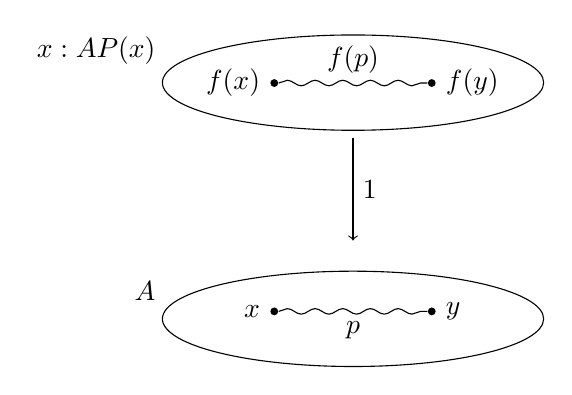
\begin{tikzpicture}[yscale=.5,xscale=2]
    \draw (0,0) arc (-90:170:8ex) node[anchor=south east] {$A$} arc (170:270:8ex);
    \draw (0,6) arc (-90:170:8ex) node[anchor=south east] {$\sm{x:A} P(x)$} arc (170:270:8ex);
    \draw[->] (0,5.8) -- node[auto] {$\proj1$} (0,3.2);
    \node[circle,fill,inner sep=1pt,label=left:{$x$}] (b1) at (-.5,1.4) {};
    \node[circle,fill,inner sep=1pt,label=right:{$y$}] (b2) at (.5,1.4) {};
    \draw[decorate,decoration={snake,amplitude=1}] (b1) -- node[auto,swap] {$p$} (b2);
    \node[circle,fill,inner sep=1pt,label=left:{$f(x)$}] (b1) at (-.5,7.2) {};
    \node[circle,fill,inner sep=1pt,label=right:{$f(y)$}] (b2) at (.5,7.2) {};
    \draw[decorate,decoration={snake,amplitude=1}] (b1) -- node[auto] {$f(p)$} (b2);
  \end{tikzpicture}
\end{center}

我们\emph{确实}可以由 \cref{lem:map} 得到这样的对象。
给定 $f:\prd{x:A} P(x)$，可定义一个非依值函数 $f':A\to \sm{x:A} P(x)$，令 $f'(x)\defeq (x,f(x))$，再考虑 $\ap{f'}{p} : f'(x) = f'(y)$。
由于 $\proj1 \circ f' \jdeq \idfunc[A]$，由 \cref{lem:ap-functor} 得 $\ap{\proj1}{\ap{f'}{p}} = p$；因此在这个意义下 $\ap{f'}{p}$ 的确“位于” $p$ 之上。
但是，仅从 $\ap{f'}{p}$ 的\emph{类型}并不明显看出它位于 $A$ 中某条特定路径（此处即 $p$）之上，而这有时很重要。

解决办法是使用传送引理。
由 \cref{thm:path-lifting}，我们有位于 $p$ 之上的规范路径 $\mathsf{lift}(u,p)$，它从 $(x,u)$ 到 $(y,\trans p u)$。
因此，任何位于 $p$ 之上、从 $u:P(x)$ 到 $v:P(y)$ 的路径，都应当通过 $\mathsf{lift}(u,p)$（本质上唯一地）分解为一条完全位于纤维 $P(y)$ 内、从 $\trans p u$ 到 $v$ 的路径。
所以，在等价意义下，把“位于 $p:x=y$ 之上、从 $u$ 到 $v$ 的路径”定义为 $P(y)$ 中的一条路径 $\trans p u = v$ 是合理的。
并且我们确实可以证明依值函数会产生这样的路径。

\begin{lem}[依值映射]\label{lem:mapdep}
  \indexdef{application!of dependent function to a path}%
  \indexdef{path!application of a dependent function to}%
  \indexdef{function!dependent!application to a path of}%
  \indexdef{action!of a dependent function on a path}%
  设 $f:\prd{x: A} P(x)$；则有映射
  \[\apdfunc f : \prd{p:x=y}\big(\id[P(y)]{\trans p{f(x)}}{f(y)}\big).\]
\end{lem}

\begin{proof}[第一种证明]
  令 $D:\prd{x,y:A} (\id{x}{y}) \to \type$ 为如下定义的类型族：
  \begin{equation*}
    D(x,y,p)\defeq \trans p {f(x)}= f(y).
  \end{equation*}
  则 $D(x,x,\refl{x})$ 为 $\trans{(\refl{x})}{f(x)}= f(x)$。
  但由于 $\trans{(\refl{x})}{f(x)}\jdeq f(x)$，可得 $D(x,x,\refl{x})\jdeq (f(x)= f(x))$。
  因而可得函数
  \begin{equation*}
    d\defeq\lam{x} \refl{f(x)}:\prd{x:A} D(x,x,\refl{x})
  \end{equation*}
  现由路径归纳可得：对每个 $p:x= y$，有
  \narrowequation{\apdfunc f(p):\trans p{f(x)}= f(y).}
\end{proof}

\begin{proof}[第二种证明]
  由归纳法，只需考虑 $p$ 为 $\refl x$。
  但此时所需等式是
  \narrowequation{\trans{(\refl{x})}{f(x)}= f(x),}
  它按判定相等成立。
\end{proof}

在这个意义下，我们将一般地把“位于其他路径之上”的路径称为\emph{依值路径}。
\indexsee{dependent!path}{path, dependent}%
\index{path!dependent}%
从 \cref{cha:hits} 开始，它们将发挥越来越重要的作用。
在 \cref{sec:computational} 中我们将看到：对某些特定类型族，依值路径概念存在等价但有时更便捷的表示方式。

现在回忆 \cref{sec:pi-types}：非依值类型函数 $f:A\to B$ 只是依值类型函数 $f:\prd{x:A} P(x)$ 的特例，其中 $P$ 是常值类型族，$P(x) \defeq B$。
在此情形下，$\apdfunc{f}$ 与 $\apfunc{f}$ 关系密切，原因见下引理：

\begin{lem}\label{thm:trans-trivial}
  若 $P:A\to\type$ 由某固定的 $B:\type$ 定义为 $P(x) \defeq B$，则对任意 $x,y:A$、$p:x=y$ 与 $b:B$，我们有路径
  \[ \transconst Bpb : \transfib P p b = b. \]
\end{lem}
\begin{proof}[第一种证明]
  固定 $b:B$，令 $D:\prd{x,y:A} (\id{x}{y}) \to \type$ 为如下定义的类型族：
  \[ D(x,y,p) \defeq (\transfib P p b = b). \]
  则 $D(x,x,\refl x)$ 为 $(\transfib P{\refl{x}}{b} = b)$，按传送计算规则它与 $(b=b)$ 判定相等。
  因此我们有函数
  \[ d \defeq \lam{x} \refl{b} : \prd{x:A} D(x,x,\refl x). \]
  现在路径归纳给出一个元素，属于
  \narrowequation{
    \prd{x,y:A}{p:x=y}(\transfib P p b = b),}
  即所求。
\end{proof}
\begin{proof}[第二种证明]
  由归纳法，只需设 $y$ 为 $x$ 且 $p$ 为 $\refl x$。
  但 $\transfib P {\refl x} b \jdeq b$，所以此时我们需证明的是 $b=b$，而这由 $\refl{b}$ 给出。
\end{proof}

因此，对任意
\narrowequation{x,y:A,\qquad p:x=y,\qquad f:A\to B,}
分别与
\narrowequation{\transconst Bp{f(x)}}
及其逆拼接，可得到函数
\begin{align}
  \big(f(x) = f(y)\big) &\to \big(\trans{p}{f(x)} = f(y)\big)\label{eq:ap-to-apd}
  \qquad\text{以及} \\
  \big(\trans{p}{f(x)} = f(y)\big) &\to \big(f(x) = f(y)\big).\label{eq:apd-to-ap}
\end{align}
事实上，这两个函数互为逆等价（其意义将在 \cref{sec:basics-equivalences} 中引入），并将 $\apfunc f (p)$ 与 $\apdfunc f (p)$ 联系起来。

\begin{lem}\label{thm:apd-const}
  对 $f:A\to B$ 与 $p:\id[A]xy$，有
  \[ \apdfunc f(p) = \transconst B p{f(x)} \ct \apfunc f (p). \]
\end{lem}
\begin{proof}[第一种证明]
  令 $D:\prd{x,y:A} (\id xy) \to \type$ 为如下定义的类型族：
  \[ D(x,y,p) \defeq \big(\apdfunc f (p) = \transconst Bp{f(x)} \ct \apfunc f (p)\big). \]
  因而有
  \[D(x,x,\refl x) \jdeq \big(\apdfunc f (\refl x) = \transconst B{\refl x}{f(x)} \ct \apfunc f ({\refl x})\big).\]
  但按定义，该类型中出现的三条路径都为 $\refl{f(x)}$，故有
  \[ \refl{\refl{f(x)}} : D(x,x,\refl x). \]
  因此，路径归纳给出一个元素属于 $\prd{x,y:A}{p:x=y} D(x,y,p)$，这正是我们所需。
\end{proof}
\begin{proof}[第二种证明]
  由归纳法，只需设 $y$ 为 $x$ 且 $p$ 为 $\refl x$。
  在此情形下，我们需证明 $\refl{f(x)} = \refl{f(x)} \ct \refl{f(x)}$，它按判定相等成立。
\end{proof}

由于 $\apdfunc{f}$ 与 $\apfunc{f}$ 的类型不同，通常为它们使用不同记号会更清晰。
% We may sometimes use a notation $\apd f p$ for $\apdfunc{f}(p)$, which is similar to the notation $\ap f p$ for $\apfunc{f}(p)$.

\index{function!dependent|)}%

到这里，我们希望读者已开始熟悉对恒等类型作归纳的证明方式。
从现在起我们不再同时给出两种证明风格，而是使用最清晰、最方便的一种（通常是第二种，更简洁）。
下面给出若干关于传送的有用引理，证明留给读者（任选上述风格）。

\begin{lem}\label{thm:transport-concat}
  给定 $P:A\to\type$，以及 $p:\id[A]xy$、$q:\id[A]yz$，并设 $u:P(x)$，则有
  \[ \trans{q}{\trans{p}{u}} = \trans{(p\ct q)}{u}. \]
\end{lem}

\begin{lem}\label{thm:transport-compose}
  对函数 $f:A\to B$ 与类型族 $P:B\to\type$，以及任意 $p:\id[A]xy$ 与 $u:P(f(x))$，有
  \[ \transfib{P\circ f}{p}{u} = \transfib{P}{\apfunc f(p)}{u}. \]
\end{lem}

\begin{lem}\label{thm:ap-transport}
  对 $P,Q:A\to \type$、函数族 $f:\prd{x:A} P(x)\to Q(x)$，以及任意 $p:\id[A]xy$ 与 $u:P(x)$，有
  \[ \transfib{Q}{p}{f_x(u)} = f_y(\transfib{P}{p}{u}). \]
\end{lem}

\index{type!family of|)}%
\index{transport|)}
\section{同伦与等价}
\label{sec:basics-equivalences}

\index{homotopy|(defstyle}%

到目前为止，我们已经看到，恒等类型 $\id[A]xy$ 可以被看作类型 $A$ 中两个元素 $x$ 与 $y$ 之间的\emph{认同}、\emph{路径}或\emph{等价}的类型。
现在我们考察\emph{函数}之间以及\emph{类型}之间合适的“认同”或“同一性”概念。
在 \cref{sec:compute-pi,sec:compute-universe} 中我们将看到，同伦类型论允许把这些概念与恒等类型的实例对应起来；但在此之前，我们需要先独立理解它们。

传统上，若两个函数在所有输入上取值相等，我们就认为它们相同。
在“命题即类型”的解释下，这提示我们：若类型 $\prd{x:A} (f(x)=g(x))$ 可居留，则两个函数 $f$ 与 $g$（可以是依值类型的）应当视为相同。
在同伦解释下，这个依值函数类型由\emph{连续}路径或\emph{函子性}等价组成，因此可看作\emph{同伦}或\emph{自然同构}的类型。\index{isomorphism!natural}
我们将采用这一拓扑术语。

\begin{defn} \label{defn:homotopy}
  设 $f,g:\prd{x:A} P(x)$ 是类型族 $P:A\to\type$ 的两个截面。
  从 $f$ 到 $g$ 的\define{同伦}
  是一个如下类型的依值函数：
  \begin{equation*}
    (f\htpy g) \defeq \prd{x:A} (f(x)=g(x)).
  \end{equation*}
\end{defn}

注意，同伦并不等同于认同 $(f=g)$。
不过在 \cref{sec:compute-pi} 中我们将引入一个公理，使同伦与认同“等价”。

下述证明留给读者。

\begin{lem}\label{lem:homotopy-props}
  对每个依值函数类型 $\prd{x:A} P(x)$，同伦构成一个等价关系。
  即我们有下列类型的元素：
  \begin{gather*}
    \prd{f:\prd{x:A} P(x)} (f\htpy f)\\
    \prd{f,g:\prd{x:A} P(x)} (f\htpy g) \to (g\htpy f)\\
    \prd{f,g,h:\prd{x:A} P(x)} (f\htpy g) \to (g\htpy h) \to (f\htpy h).
  \end{gather*}
\end{lem}

% This is judgmental and is \cref{ex:composition}.
% \begin{lem}
%   Composition is associative and unital up to homotopy.
%   That is:
%   \begin{enumerate}
%   \item If $f:A\to B$ then $f\circ \idfunc[A]\htpy f\htpy \idfunc[B]\circ f$.
%   \item If $f:A\to B, g:B\to C$ and $h:C\to D$ then $h\circ (g\circ f) \htpy (h\circ g)\circ f$.
%   \end{enumerate}
% \end{lem}

\index{functoriality of functions in type theory@``functoriality'' of functions in type theory}%
\index{continuity of functions in type theory@``continuity'' of functions in type theory}%
正如类型论中的函数自动是“函子”一样，同伦也自动是
\index{naturality of homotopies@``naturality'' of homotopies}%
“自然变换”。
我们只对非依值函数 $f,g:A\to B$ 陈述并证明这一点；在 \cref{ex:dep-htpy-natural} 中我们请读者将其推广到依值函数。

回忆：对 $f:A\to B$ 与 $p:\id[A]xy$，我们可写 $\ap f p$ 表示 $\apfunc{f} (p)$。

\begin{lem}\label{lem:htpy-natural}
  设 $H:f\htpy g$ 是函数 $f,g:A\to B$ 之间的同伦，且 $p:\id[A]xy$。
  则有
  \begin{equation*}
    H(x)\ct\ap{g}{p}=\ap{f}{p}\ct H(y).
  \end{equation*}
  我们也可将其画成交换图：\index{diagram}
  \begin{align*}
    \xymatrix{
      f(x) \ar@{=}[r]^{\ap fp} \ar@{=}[d]_{H(x)} & f(y) \ar@{=}[d]^{H(y)} \\
      g(x) \ar@{=}[r]_{\ap gp} & g(y)
    }
  \end{align*}
\end{lem}
\begin{proof}
  由归纳法，可设 $p$ 为 $\refl x$。
  由于 $\apfunc{f}$ 与 $\apfunc g$ 在反身性上可计算，此时我们需证明
  \[ H(x) \ct \refl{g(x)} = \refl{f(x)} \ct H(x). \]
  这成立，因为两边都等于 $H(x)$。
\end{proof}

\begin{cor}\label{cor:hom-fg}
  令 $H : f \htpy \idfunc[A]$ 为一个同伦，其中 $f : A \to A$。则对任意 $x : A$，有 \[ H(f(x)) = \ap f{H(x)}. \]
  % The above path will be denoted by $\com{H}{f}{x}$.
\end{cor}
\noindent
这里 $f(x)$ 表示 $f$ 对 $x$ 的通常作用，而 $\ap f{H(x)}$ 表示 $\apfunc{f}(H(x))$。
\begin{proof}
由 $H$ 的自然性，下面的路径图交换：
\begin{align*}
\xymatrix@C=3pc{
ffx \ar@{=}[r]^-{\ap f{Hx}} \ar@{=}[d]_{H(fx)} & fx \ar@{=}[d]^{Hx} \\
fx \ar@{=}[r]_-{Hx} & x
}
\end{align*}
也就是说，$\ap f{H x} \ct H x = H(f x) \ct H x$。
现在将 $\opp{(H x)}$ 作 whisker 以消去 $H x$，得到
\[ \ap f{H x}
= \ap f{H x} \ct H x \ct \opp{(H x)}
= H(f x) \ct H x \ct \opp{(H x)}
= H(f x)
\]
即得所求（其中省略了一些结合性的路径）。
\end{proof}

当然，和函数的函子性（\cref{lem:ap-functor}）一样，\cref{lem:htpy-natural} 中的等式本身也是一条路径，并满足其自身的一致性律，等等。

\index{homotopy|)}%

\index{equivalence|(}%
转到类型层面，从传统观点可说：若存在函数 $g:B\to A$ 使得两个复合 $f\circ g$ 与 $g\circ f$ 都逐点等于恒等函数，即满足 $f \circ g \htpy \idfunc[B]$ 且 $g\circ f \htpy \idfunc[A]$，则函数 $f:A\to B$ 是一个\emph{同构}。
\indexsee{homotopy!equivalence}{equivalence}%
同伦观点提示这应称为\emph{同伦等价}；从范畴论观点看，应称为（高阶）群胚的\emph{等价}。
然而，在做证明相关数学时，
\index{mathematics!proof-relevant}%
对应的类型
\begin{equation}
  \sm{g:B\to A} \big((f \circ g \htpy \idfunc[B]) \times (g\circ f \htpy \idfunc[A])\big)\label{eq:qinvtype}
\end{equation}
表现并不好。
例如，对同一个函数 $f:A\to B$，\eqref{eq:qinvtype} 可能有多个彼此不相等的居留元。
（这与高阶范畴论中的一个观察密切相关：通常需要考虑\emph{伴随}等价\index{adjoint!equivalence}，而非朴素等价。）
因此，我们给 \eqref{eq:qinvtype} 取如下名称：它在历史上准确，但语气略带贬义。

\begin{defn}\label{defn:quasi-inverse}
  对函数 $f:A\to B$，$f$ 的一个\define{拟逆}
  \indexdef{quasi-inverse}%
  \indexsee{function!quasi-inverse of}{quasi-inverse}%
  是三元组 $(g,\alpha,\beta)$，其中 $g:B\to A$ 是函数，且
$\alpha:f\circ g\htpy \idfunc[B]$ 与 $\beta:g\circ f\htpy \idfunc[A]$ 是同伦。
\end{defn}

\symlabel{qinv}
因此，\eqref{eq:qinvtype} 就是\emph{$f$ 的拟逆类型}；可记为 $\qinv(f)$。

\begin{eg}\label{eg:idequiv}
  \index{identity!function}%
  \index{function!identity}%
  恒等函数 $\idfunc[A]:A\to A$ 具有一个拟逆，即其自身 $\idfunc[A]$，并配以同伦 $\alpha(y) \defeq \refl{y}$ 与 $\beta(x) \defeq \refl{x}$。
\end{eg}

\begin{eg}\label{eg:concatequiv}
  对任意 $p:\id[A]xy$ 与 $z:A$，函数
  \begin{align*}
    (p\ct \blank)&:(\id[A]yz) \to (\id[A]xz) \qquad\text{以及}\\
    (\blank \ct p)&:(\id[A]zx) \to (\id[A]zy)
  \end{align*}
  分别具有拟逆 $(\opp p \ct \blank)$ 与 $(\blank \ct \opp p)$；见 \cref{ex:equiv-concat}。
\end{eg}

\begin{eg}\label{thm:transportequiv}
  对任意 $p:\id[A]xy$ 与 $P:A\to\type$，函数
  \[\transfib{P}{p}{\blank}:P(x) \to P(y)\]
  具有一个拟逆 $\transfib{P}{\opp p}{\blank}$；这可由 \narrowbreak \cref{thm:transport-concat} 得到。
\end{eg}

\symlabel{basics-isequiv}\symlabel{basics:iso}
一般而言，我们只在类型 $A$ 与 $B$“表现得像集合”时（见 \cref{sec:basics-sets}）使用\emph{同构}
\index{isomorphism!of sets}
（以及类似词语如\emph{双射}，及相应记号 $A\cong B$）
\index{bijection}
一词。
在这种情形下，类型 \eqref{eq:qinvtype} 没有问题。
我们保留“\emph{等价}”一词给改进后的概念 $\isequiv (f)$，它应满足下列性质：%
\begin{enumerate}
\item 对每个 $f:A\to B$，存在函数 $\qinv(f) \to \isequiv (f)$。\label{item:be1}
\item 同样地，对每个 $f$，有 $\isequiv (f) \to \qinv(f)$；因此两者在逻辑上等价（见 \cref{sec:pat}）。\label{item:be2}
\item 对任意两个居留元 $e_1,e_2:\isequiv(f)$，有 $e_1=e_2$。\label{item:be3}
\end{enumerate}
在 \cref{cha:equivalences} 中我们将看到：满足这三条性质的 $\isequiv(f)$ 有许多不同定义，但彼此都等价。
目前为使读者相信这类定义确实存在，我们只给出其中最容易的一个：
\begin{equation}\label{eq:isequiv-invertible}
  \isequiv(f) \;\defeq\;
  \Parens{\sm{g:B\to A} (f\circ g \htpy \idfunc[B])}
  \times
  \Parens{\sm{h:B\to A} (h\circ f \htpy \idfunc[A])}.
\end{equation}
对这个定义，我们现在可证明性质 \ref{item:be1} 与 \ref{item:be2}。
函数 $\qinv(f) \to \isequiv (f)$ 很容易定义：将 $(g,\alpha,\beta)$ 送到 $(g,\alpha,g,\beta)$。
反向地，给定 $(g,\alpha,h,\beta)$，令 $\gamma$ 为复合同伦
\[ g \overset{\beta}{\htpy} h\circ f\circ g \overset{\alpha}{\htpy} h, \]
其含义是 $\gamma(x) \defeq \opp{\beta(g(x))} \ct \ap{h}{\alpha(x)}$。
现在定义 $\beta':g\circ f\htpy \idfunc[A]$ 为 $\beta'(x) \defeq \gamma(f(x)) \ct \beta(x)$。
则 $(g,\alpha,\beta'):\qinv(f)$。

对该定义，性质 \ref{item:be3} 的证明也不太难，但它需要识别笛卡尔积类型与依值二元组类型的恒等类型，这将在 \cref{sec:compute-cartprod,sec:compute-sigma} 讨论。
因此我们也将其推迟；见 \cref{sec:biinv}。
此时最重要的结论是：存在一个行为良好的类型，可读作“$f$ 是一个等价”；并且只要给出一个拟逆，就能证明 $f$ 是等价。
在实践中，这是证明函数为等价的最常用方式。

按照证明相关哲学，
\index{mathematics!proof-relevant}%
从 $A$ 到 $B$ 的\emph{一个等价}被定义为函数 $f:A\to B$ 连同 $\isequiv (f)$ 的一个居留元，即它是等价的证明。
我们记 $(\eqv A B)$ 为从 $A$ 到 $B$ 的等价类型，即
\begin{equation}\label{eq:eqv}
  (\eqv A B) \defeq \sm{f:A\to B} \isequiv(f).
\end{equation}
上述性质 \ref{item:be3} 将保证：若两个等价作为函数相等（即它们作为 $A\to B$ 的底层元素相等），则它们作为等价也相等（见 \cref{sec:compute-sigma}）。
因此，我们常常略去区分等价与其底层函数。
例如，若有函数 $f:A\to B$ 且知 $e:\isequiv(f)$，我们可写 $f:\eqv A B$，而不写 $\tup{f}{e}$。
反之，若有等价 $g:\eqv A B$，给定 $a:A$ 时可写 $g(a)$，而不写 $(\proj1 g)(a)$。

最后我们指出：

\begin{lem}\label{thm:equiv-eqrel}
  类型等价是 \type 上的一个等价关系。
  更具体地：
  \begin{enumerate}
  \item 对任意 $A$，恒等函数 $\idfunc[A]$ 是等价；因此有 $\eqv A A$。
  \item 对任意 $f:\eqv A B$，有等价 $f^{-1} : \eqv B A$。
  \item 对任意 $f:\eqv A B$ 与 $g:\eqv B C$，有 $g\circ f : \eqv A C$。
  \end{enumerate}
\end{lem}
\begin{proof}
  恒等函数显然是它自身的拟逆；因此它是等价。

  若 $f:A\to B$ 是等价，则它有一个拟逆，记作 $f^{-1}:B\to A$。
  那么 $f$ 也是 $f^{-1}$ 的拟逆，因此 $f^{-1}$ 是一个等价 $B\to A$。

  最后，给定 $f:\eqv A B$ 与 $g:\eqv B C$，其拟逆分别为 $f^{-1}$ 与 $g^{-1}$。则对任意 $a:A$，有 $f^{-1} g^{-1} g f a = f^{-1} f a = a$；对任意 $c:C$，有 $g f f^{-1} g^{-1} c = g g^{-1} c = c$。
  因此 $f^{-1} \circ g^{-1}$ 是 $g\circ f$ 的拟逆，故后者是等价。
\end{proof}

\index{equivalence|)}%
\section{类型构造子的高阶群胚结构}
\label{sec:computational}

在 \cref{cha:typetheory} 中，我们介绍了许多构造新类型的方法：笛卡尔积、不交并、依值积、依值和等。
在 \cref{sec:equality,sec:functors,sec:fibrations} 中，我们看到同伦类型论中的\emph{所有}类型都像空间或高阶群胚一样运作。
本章余下部分的目标，是把这种高阶结构在 \cref{cha:typetheory} 所定义的各类具体类型上的行为明确写出。

事实证明，对许多类型 $A$，恒等类型 $\id[A]xy$ 都可按构造 $A$ 所用的数据来刻画（在等价意义下）。
例如，若 $A$ 是笛卡尔积 $B\times C$，且 $x\jdeq (b,c)$、$y\jdeq(b',c')$，则有等价
\begin{equation}\label{eq:prodeqv}
  \eqv{\big((b,c)=(b',c')\big)}{\big((b=b')\times (c=c')\big)}.
\end{equation}
用更传统的语言说，两有序对相等当且仅当其分量分别相等（但等价式 \eqref{eq:prodeqv} 的内容比这更多）。
恒等类型的高阶结构也可用这些等价来表达；例如，两条“对偶之间的相等”之拼接，对应于分量逐一拼接。

类似地，当类型族 $P:A\to\type$ 逐纤维地由 \cref{cha:typetheory} 的类型构造规则搭建而成时，操作 $\transfib{P}{p}{\blank}$ 也可按构成 $P$ 的数据上的对应操作来刻画（到同伦为止）。
例如，若 $P(x) \jdeq B(x)\times C(x)$，则有
\[\transfib{P}{p}{(b,c)} = \big(\transfib{B}{p}{b},\transfib{C}{p}{c}\big).\]

最后，类型构造规则本身也是函子性的；若函数 $f$ 是由这种函子性构造而来，则 $\apfunc f$ 与 $\apdfunc f$ 的操作可由构成 $f$ 的数据上的对应操作来计算。
例如，若 $g:B\to B'$、$h:C\to C'$，并定义 $f:B\times C \to B'\times C'$ 为 $f(b,c)\defeq (g(b),h(c))$，则在等价式 \eqref{eq:prodeqv} 的意义下，可将 $\apfunc f$ 识别为“$(\apfunc g,\apfunc h)$”。

接下来的几节（\crefrange{sec:compute-cartprod}{sec:compute-nat}）将逐一针对每个基本类型构造子，陈述并证明这类定理。
在这里我们会遇到当前可用类型论中的一个表面缺陷；
正如后续章节将更清楚地展示的那样，若这些关于恒等类型、传送等的刻画是\emph{判定}\index{judgmental equality}等式，会更方便也更直观。
然而，在 \cref{cha:typetheory} 给出的理论中，恒等类型由其归纳原理对所有类型统一定义，因此我们不能在不同类型处把它们“重定义”为不同对象。
所以，本章讨论的针对特定类型的刻画，大多是我们必须去发现并证明（若可能）的\emph{定理}。

实际上，\cref{cha:typetheory} 的类型论不足以证明两类构造子的所需定理：$\Pi$-类型与宇宙。
因此，我们不得不向类型论中引入公理，才能使那些“定理”成立。
从类型论角度看，\emph{公理}（参见 \cref{sec:axioms}）是一个“原子”元素：它被声明为某指定类型的居留元，但除它所居留类型的一般规则外，并无额外行为规则。
\index{axiom!versus rules}%

\index{function extensionality}%
\indexsee{extensionality, of functions}{function extensionality}
\index{univalence axiom}%
针对 $\Pi$-类型的公理（\cref{sec:compute-pi}）对类型论学者并不陌生：它称为\emph{函数外延性}，其大意是若两个函数在 \cref{sec:basics-equivalences} 的意义下同伦，则它们相等。
而针对宇宙的公理（\cref{sec:compute-universe}）则是同伦类型论由 Voevodsky 提出的新贡献：它称为\emph{泛等公理}，其大意是若两个类型在 \cref{sec:basics-equivalences} 的意义下等价，则它们相等。
我们已在导言中提到该公理；它将在本书中发挥非常重要的作用。%
\footnote{我们选择将这些原理作为公理引入，但也可能存在其他方式来表述一种使其成立的类型论。
  见本章注记。}

需要强调的是，并非\emph{所有}恒等类型都能通过对类型构造的归纳来“确定”。
反例包括大多数非平凡高阶归纳类型（见 \cref{cha:hits,cha:homotopy}）。
例如，计算类型 $\Sn^n$ 的恒等类型（见 \cref{sec:circle}）等价于计算球面的高阶同伦群，而这在代数拓扑中是一个深刻且重要的研究领域。

\section{笛卡尔乘积类型}
\label{sec:compute-cartprod}

\index{type!product|(}%
给定类型 $A$ 和 $B$，考虑笛卡尔乘积类型 $A \times B$。
对任意元素 $x,y:A\times B$ 与路径 $p:\id[A\times B]{x}{y}$，由函子性可提取路径 $\ap{\proj1}p:\id[A]{\proj1(x)}{\proj1(y)}$ 和 $\ap{\proj2}p:\id[B]{\proj2(x)}{\proj2(y)}$。
因此，我们有一个函数
\begin{equation}\label{eq:path-prod}
  (\id[A\times B]{x}{y}) \to (\id[A]{\proj1(x)}{\proj1(y)}) \times (\id[B]{\proj2(x)}{\proj2(y)}).
\end{equation}

\begin{thm}\label{thm:path-prod}
  对任意 $x$ 和 $y$，函数~\eqref{eq:path-prod} 是一个等价。
\end{thm}

从逻辑上读，这表示两个有序对相等当且仅当其分量分别相等。
从范畴论上读，这表示积群胚中的态射是态射对。
从同伦论上读，这表示积空间中的路径是路径对。

\begin{proof}
  我们需要构造反方向的函数：
  \begin{equation}
    (\id[A]{\proj1(x)}{\proj1(y)}) \times (\id[B]{\proj2(x)}{\proj2(y)}) \to (\id[A\times B]{x}{y}). \label{eq:path-prod-inverse}
  \end{equation}
  由笛卡尔乘积的归纳法则，可设 $x$ 与 $y$ 都是有序对，即对某些 $a,a':A$ 和 $b,b':B$，有 $x\jdeq (a,b)$ 与 $y\jdeq (a',b')$。
  在这种情况下，我们需要的是函数
  \begin{equation*}
    (\id[A]{a}{a'}) \times (\id[B]{b}{b'}) \to \big(\id[A\times B]{(a,b)}{(a',b')}\big).
  \end{equation*}
  再由其定义域上的笛卡尔乘积归纳，可设给定 $p:a=a'$ 和 $q:b=b'$。
  再做两次路径归纳，可设 $a\jdeq a'$ 且 $b\jdeq b'$，并且 $p,q$ 都是自反性。
  此时 $(a,b)\jdeq(a',b')$，因此输出也可取自反性。

  还需证明~\eqref{eq:path-prod-inverse} 与~\eqref{eq:path-prod} 互为拟逆。
  这是一串直接的归纳，但顺序必须正确。

  一个方向上，从 $r:\id[A\times B]{x}{y}$ 开始。
  先对 $r$ 作路径归纳，可设 $x\jdeq y$ 且 $r$ 为自反性。
  在这种情况下，由于 $\apfunc{\proj1}$ 和 $\apfunc{\proj2}$ 由路径归纳定义，~\eqref{eq:path-prod} 将 $r\jdeq \refl{x}$ 送到有序对 $(\refl{\proj1x},\refl{\proj2x})$。
  现在再对 $x$ 归纳，可设 $x\jdeq (a,b)$，于是这就是 $(\refl a, \refl b)$。
  因而，~\eqref{eq:path-prod-inverse} 按定义将其送到 $\refl{(a,b)}$，在当前假设下即为 $r$。

  另一个方向上，若从 $s:(\id[A]{\proj1(x)}{\proj1(y)}) \times (\id[B]{\proj2(x)}{\proj2(y)})$ 开始，则先对 $x,y$ 归纳，设其为有序对 $(a,b)$ 和 $(a',b')$，再对 $s:(\id[A]{a}{a'}) \times (\id[B]{b}{b'})$ 归纳，将其化为有序对 $(p,q)$，其中 $p:a=a'$、$q:b=b'$。
  现在对 $p,q$ 归纳，可设其为自反性 $\refl a$ 与 $\refl b$；此时~\eqref{eq:path-prod-inverse} 给出 $\refl{(a,b)}$，再经~\eqref{eq:path-prod} 返回 $(\refl a,\refl b)\jdeq (p,q)\jdeq s$。
\end{proof}

特别地，我们已证明~\eqref{eq:path-prod} 有逆~\eqref{eq:path-prod-inverse}，记为
\symlabel{defn:pairpath}
\[
\pairpath : (\id{\proj{1}(x)}{\proj{1}(y)}) \times (\id{\proj{2}(x)}{\proj{2}(y)}) \to (\id x y).
\]
注意其特例给出了乘积类型的命题唯一性原理\index{uniqueness!principle, propositional!for product types}：$z = (\proj1(z),\proj2(z))$。

将 \pairpath 视作 $\id x y$ 的一个\emph{构造子}或\emph{引入规则}会很有帮助，它类似于 $A\times B$ 自身的“配对”构造子：在给定 $a:A$ 与 $b:B$ 时引入有序对 $(a,b)$。
从这个角度看，~\eqref{eq:path-prod} 的两个分量：
\begin{align*}
  \projpath{1} &: (\id{x}{y}) \to (\id{\proj{1}(x)}{\proj{1} (y)})\\
  \projpath{2} &: (\id{x}{y}) \to (\id{\proj{2}(x)}{\proj{2} (y)})
\end{align*}
是\emph{消去}规则。
类似地，见证~\eqref{eq:path-prod-inverse} 是~\eqref{eq:path-prod} 拟逆的两个同伦，分别由\emph{命题计算规则}组成：
\index{computation rule!propositional!for identities between pairs}%
\begin{align*}
  {\projpath{1}{(\pairpath(p, q)})}
  &= %_{(\id{\proj{1} x}{\proj{1} y})}
  {p} \\
  {\projpath{2}{(\pairpath(p,q)})}
  &= %_{(\id{\proj{2} x}{\proj{2} y})}
  {q}
\end{align*}
其中 $p:\id{\proj{1} x}{\proj{1} y}$ 且 $q:\id{\proj{2} x}{\proj{2} y}$，
以及一个\emph{命题唯一性原理}：
\index{uniqueness!principle, propositional!for identities between pairs}%
\[
\id{r}{\pairpath(\projpath{1} (r), \projpath{2} (r)) }
\qquad\text{for } r : \id[A \times B] x y.
\]

我们还可逐分量刻画 $A\times B$ 中路径的自反性、逆与复合：
\begin{align*}
  {\refl{(z : A \times B)}}
  &= {\pairpath (\refl{\proj{1} z},\refl{\proj{2} z})} \\
  {\opp{p}}
  &= {\pairpath \big(\opp{\projpath{1} (p)},\, \opp{\projpath{2} (p)}\big)} \\
  {{p \ct q}}
  &= {\pairpath \big({\projpath{1} (p)} \ct {\projpath{1} (q)},\,{\projpath{2} (p)} \ct {\projpath{2} (q)}\big)}.
\end{align*}
或写成：
\begin{alignat*}{2}
  \projpath{i}(\refl{(z : A \times B)}) &= \refl{\proj{i} z} &\qquad (i=1,2)\\
  \pairpath(\opp p, \opp q) &= \opp{\pairpath(p,q)}\\
  \pairpath(p\ct q, p'\ct q') &= \pairpath(p,p') \ct \pairpath(q,q').
\end{alignat*}
这些等式都可通过对给定路径作路径归纳并返回自反性得到。
对 \cref{sec:equality} 中其余高阶群胚结构也同样成立，不过要插入足够多的其他相干路径来得到可通过类型检查的等式会变得繁琐。
例如，若将 \cref{thm:omg}\ref{item:omg4} 中路径的逆记为 $\ctassoc(p,q,r)$，并将上面最后展示的路径记为 $\pairct(p,q,p',q')$，则对任意 $u,v,z,w:A\times B$ 以及适当类型的 $p,q,r,p',q',r'$，有
\begin{equation*}
  \begin{array}{l}
    \pairct(p\ct q, r, p'\ct q', r') \\
    \ct\;  (\pairct(p,q,p',q') \rightwhisker \pairpath(r,r')) \\
    \ct\;  \ctassoc(\pairpath(p,p'),\pairpath(q,q'),\pairpath(r,r'))\\
    =
    \begin{array}[t]{l}
      \apfunc{\pairpath}({\pairpath(\ctassoc(p,q,r),\ctassoc(p',q',r'))})\\
      \ct\; \pairct(p, q\ct r, p', q'\ct r')\\
      \ct\; (\pairpath(p,p') \leftwhisker \pairct(q,r,q',r')).
    \end{array}
  \end{array}
\end{equation*}
幸运的是，我们永远不需要使用这类更高维的相干性。

\index{transport!in product types}%
现在考虑类型族逐点乘积中的传送。
给定类型族 $ A, B : Z \to \type$，我们滥用记号写 $A\times B:Z\to \type$ 表示由 $(A\times B)(z) \defeq A(z) \times B(z)$ 定义的类型族。
现给定 $p : \id[Z]{z}{w}$ 与 $x : A(z) \times B(z)$，可沿 $p$ 传送 $x$ 以得到 $A(w)\times B(w)$ 的元素。

\begin{thm}\label{thm:trans-prod}
  在上述情形中，有
  \[
  \id[A(w) \times B(w)]
  {\transfib{A\times B}px}
  {(\transfib{A}{p}{\proj{1}x}, \transfib{B}{p}{\proj{2}x})}.
  \]
\end{thm}
\begin{proof}
  由路径归纳，可设 $p$ 为自反性，此时
  \begin{align*}
    \transfib{A\times B}px&\jdeq x\\
    \transfib{A}{p}{\proj{1}x}&\jdeq \proj1x\\
    \transfib{B}{p}{\proj{2}x}&\jdeq \proj2x.
  \end{align*}
  因而只需证明 $x = (\proj1 x, \proj2x)$。
  但这正是乘积类型的命题唯一性原理；正如上文所述，它可由 \cref{thm:path-prod} 推出。
\end{proof}

最后考虑笛卡尔乘积下 $\apfunc{}$ 的函子性。
设给定类型 $A,B,A',B'$ 与函数 $g:A\to A'$、$h:B\to B'$；于是可定义函数 $f:A\times B\to A'\times B'$，其定义为 $f(x) \defeq (g(\proj1x),h(\proj2x))$。

\begin{thm}\label{thm:ap-prod}
  在上述情形中，给定 $x,y:A\times B$ 与 $p:\proj1x=\proj1y$ 以及 $q:\proj2x=\proj2y$，有
  \[ \id[(f(x)=f(y))]{\ap{f}{\pairpath(p,q)}} {\pairpath(\ap{g}{p},\ap{h}{q})}. \]
\end{thm}
\begin{proof}
  先注意上式类型良构。
  一方面，由于 $\pairpath(p,q):x=y$，故有 $\ap{f}{\pairpath(p,q)}:f(x)=f(y)$。
  另一方面，由于 $\proj1(f(x))\jdeq g(\proj1x)$ 且 $\proj2(f(x))\jdeq h(\proj2x)$，也有 $\pairpath(\ap{g}{p},\ap{h}{q}):f(x)=f(y)$。

  现在由归纳可设 $x\jdeq(a,b)$ 与 $y\jdeq(a',b')$，此时 $p:a=a'$ 且 $q:b=b'$。
  因而由路径归纳可设 $p,q$ 都是自反性，此时所需等式在判断上成立。
\end{proof}

\index{type!product|)}%

\section{\texorpdfstring{$\Sigma$}{Σ}-类型}
\label{sec:compute-sigma}

\index{type!dependent pair|(}%
设 $A$ 是一个类型，$P:A\to\type$ 是一个类型族。
回忆 $\Sigma$-类型（即依值对类型）$\sm{x:A} P(x)$ 是笛卡尔乘积类型的推广。
因此，我们也期待其高阶群胚结构是上一节结果的推广。
特别地，其中的路径应当是路径对，但要给出这些路径的正确类型仍需一些思考。

设在 $\sm{x:A}P(x)$ 中有一条路径 $p:w=w'$。
则得到 $\ap{\proj{1}}{p}:\proj{1}(w)=\proj{1}(w')$。
然而我们不能直接询问 $\proj{2}(w)$ 是否与 $\proj{2}(w')$ 相同，因为它们未必属于同一类型。
但我们可以沿路径 $\ap{\proj{1}}{p}$ 传送\index{transport} $\proj{2}(w)$，这确实会给出与 $\proj{2}(w')$ 同类型的元素。
由路径归纳，实际上可得到路径 $\trans{\ap{\proj{1}}{p}}{\proj{2}(w)}=\proj{2}(w')$。

回忆 \cref{lem:mapdep} 之前的讨论，
\narrowequation{
  \trans{\ap{\proj{1}}{p}}{\proj{2}(w)}=\proj{2}(w')
}
可视作从 $\proj2(w)$ 到 $\proj2(w')$ 且覆盖 $A$ 中路径 $\ap{\proj1}{p}$ 的路径类型。
\index{fibration}%
\index{total!space}%
因此，我们是在说：总空间中的一条路径 $w=w'$ 决定（且被决定于）$A$ 中的一条路径 $p:\proj1(w)=\proj1(w')$，以及一条从 $\proj2(w)$ 到 $\proj2(w')$ 且覆盖 $p$ 的路径，这很合理。

\begin{rmk}\label{rmk:sigma-equality-extraction}
  注意，若有 $x:A$ 和 $u,v:P(x)$ 满足 $(x,u)=(x,v)$，并不能推出 $u=v$；反例见 \cref{ex:sigma-eq-components-neq}。
  我们最多只能推出存在 $p:x=x$ 使得 $\trans p u = v$。
  这对类型论初学者是常见困惑来源，但从拓扑视角看是合理的：在纤维化总空间中，两点恰好位于同一纤维时，存在路径 $(x,u)=(x,v)$ 并不蕴含存在完全位于该纤维\emph{内部}的路径 $u=v$。
\end{rmk}

下一个定理说明这个过程也可逆。
由于它是 \cref{thm:path-prod} 的直接推广，我们将更简洁地叙述。

\begin{thm}\label{thm:path-sigma}
设 $P:A\to\type$ 是类型 $A$ 上的一个类型族，且 $w,w':\sm{x:A}P(x)$。则有一个等价
\begin{equation*}
\eqvspaced{(w=w')}{\dsm{p:\proj{1}(w)=\proj{1}(w')} \trans{p}{\proj{2}(w)}=\proj{2}(w')}.
\end{equation*}
\end{thm}

\begin{proof}
我们先定义函数
\begin{equation*}
f : \prd{w,w':\sm{x:A}P(x)} (w=w') \to \dsm{p:\proj{1}(w)=\proj{1}(w')} \trans{p}{\proj{2}(w)}=\proj{2}(w')
\end{equation*}
为路径归纳给出，满足
\begin{equation*}
f(w,w,\refl{w})\defeq(\refl{\proj{1}(w)},\refl{\proj{2}(w)}).
\end{equation*}
我们要证明 $f$ 是等价。

反方向上，定义
\begin{narrowmultline*}
  g : \prd{w,w':\sm{x:A}P(x)}
      \Parens{\sm{p:\proj{1}(w)=\proj{1}(w')}\trans{p}{\proj{2}(w)}=\proj{2}(w')}
      \to
      \narrowbreak
      (w=w')
\end{narrowmultline*}
先对 $w,w'$ 归纳，把它们分别拆成 $(w_1,w_2)$ 与
$(w_1',w_2')$，于是只需证明
\begin{equation*}
\Parens{\sm{p:w_1 = w_1'}\trans{p}{w_2}=w_2'} \to ((w_1,w_2)=(w_1',w_2')).
\end{equation*}
接着，给定一对 $\sm{p:w_1 = w_1'}\trans{p}{w_2}=w_2'$，可
用 $\Sigma$-归纳得到 $p : w_1 = w_1'$ 与 $q :
\trans{p}{w_2}=w_2'$。再对 $p$ 归纳后，有 $q :
\trans{(\refl{w_1})}{w_2}=w_2'$，只需证明
$(w_1,w_2)=(w_1,w_2')$。但 $\trans{(\refl{w_1})}{w_2} \jdeq w_2$，故
再对 $q$ 归纳可将目标化为
$(w_1,w_2)=(w_1,w_2)$，用 $\refl{(w_1,w_2)}$ 即可证明。

接着证明对所有 $w,w',r$，都有 $f(g(r))=r$，
其中 $r$ 的类型为
\[\dsm{p:\proj{1}(w)=\proj{1}(w')} (\trans{p}{\proj{2}(w)}=\proj{2}(w')).\]
先像定义 $g$ 那样，通过有序对归纳拆开 $w,w',r$，再做两次路径归纳，
把 $r$ 的两个分量都化为 \refl{}。此时只需证明
$f (g(\refl{w_1},\refl{w_2})) = (\refl{w_1},\refl{w_2})$，它按定义成立。

同理，为证明对所有 $w,w',p:w=w'$ 都有 $g(f(p))=p$，
先对 $p$ 做路径归纳，再做有序对归纳拆开 $w$，此时只需证明
$g(f (\refl{(w_1,w_2)})) = \refl{(w_1,w_2)}$，这同样按定义成立。

因此，$f$ 有拟逆，从而是一个等价。
\end{proof}

与笛卡尔乘积情形一样，我们可把命题唯一性原理作为一个特例推出。

\begin{cor}\label{thm:eta-sigma}
  \index{uniqueness!principle, propositional!for dependent pair types}%
  对于 $z:\sm{x:A} P(x)$，有 $z = (\proj1(z),\proj2(z))$。
\end{cor}
\begin{proof}
  我们有 $\refl{\proj1(z)} : \proj1(z) = \proj1(\proj1(z),\proj2(z))$，故由 \cref{thm:path-sigma}，只需给出路径 $\trans{(\refl{\proj1(z)})}{\proj2(z)} = \proj2(\proj1(z),\proj2(z))$。
  但两边在判断上都等于 $\proj2(z)$。
\end{proof}

与二元笛卡尔乘积类似，我们可将
\cref{thm:path-sigma} 的反向映射视为
一个引入形式（\pairpath{}{}），正向映射视为
消去形式（\projpath{1} 与 \projpath{2}），而该等价
给出了相应的命题计算规则与唯一性原理。

注意，在 \cref{thm:path-lifting} 中定义的 $p:x=y$ 在 $u:P(x)$ 处的提升路径 $\mathsf{lift}(u,p)$，可识别为该引入形式的特例
\[\pairpath(p,\refl{\trans p u}):(x,u) = (y,\trans p u).\]
\index{transport!in dependent pair types}%
这会出现在 $\Sigma$-类型上传送作用的陈述中，它也是二元笛卡尔乘积情形的推广：

\begin{thm}\label{transport-Sigma}
  设有类型族
  %
  \begin{equation*}
    P:A\to\type
    \qquad\text{and}\qquad
    Q:\Parens{\sm{x:A} P(x)}\to\type.
  \end{equation*}
  %
  则可构造 $A$ 上的类型族
  \begin{equation*}
    x \mapsto \sm{u:P(x)} Q(x,u).
  \end{equation*}
  对任意路径 $p:x=y$ 及任意 $(u,z):\sm{u:P(x)} Q(x,u)$，有
  \begin{equation*}
    \trans{p}{u,z}=\big(\trans{p}{u},\,\trans{\pairpath(p,\refl{\trans pu})}{z}\big).
  \end{equation*}
\end{thm}

\begin{proof}
由路径归纳立得。
\end{proof}

我们将 \cref{thm:ap-prod} 的推广（见 \cref{ex:ap-sigma}）以及
$\Sigma$-类型中路径的自反性、逆与复合的逐分量刻画
留给读者陈述并证明。

\index{type!dependent pair|)}%

\section{单位类型}
\label{sec:compute-unit}

\index{type!unit|(}%
平凡情形有时也很重要，因此我们简要讨论单位类型~\unit 的情形。

\begin{thm}\label{thm:path-unit}
  对任意 $x,y:\unit$，有 $\eqv{(x=y)}{\unit}$。
\end{thm}

一种自然想法是先对 $x,y$ 作 $\unit$-归纳，把问题化为 $\eqv{(\ttt=\ttt)}{\unit}$。
但此时会卡住，因为我们无法对 $p:\ttt=\ttt$ 再作路径归纳。
因此我们尽可能长时间保持一般的 $x,y$，只在最后一步才用归纳把它们化为 $\ttt$。

\begin{proof}
  函数 $(x=y)\to\unit$ 很容易定义：把所有输入都送到 \ttt。
  反过来，对任意 $x,y:\unit$，可由归纳设 $x\jdeq \ttt\jdeq y$。
  在此情形下有 $\refl{\ttt}:x=y$，从而得到常值函数 $\unit\to(x=y)$。

  为证明二者互逆，先取元素 $u:\unit$。
  可设 $u\jdeq\ttt$，而这也是复合 $\unit \to (x=y)\to\unit$ 的结果。

  另一方面，设给定 $p:x=y$。
  由路径归纳可设 $x\jdeq y$ 且 $p$ 为 $\refl x$。
  继而可设 $x$ 为 \ttt，此时复合 $(x=y) \to \unit\to(x=y)$ 将 $p$ 送到 $\refl x$，也即送回~$p$。
\end{proof}

特别地，\unit 的任意两个元素都相等。
我们把该等价按引入、消去、计算与唯一性规则来表述的工作留给读者。
\index{transport!in unit type}%
\unit 的传送引理就是常值类型族的传送引理（\cref{thm:trans-trivial}）。

\index{type!unit|)}%

\section{\texorpdfstring{$\Pi$}{Π}-类型与函数外延性公理}
\label{sec:compute-pi}

\index{type!dependent function|(}%
\index{type!function|(}%
\index{homotopy|(}%
给定一个类型 $A$ 和一个类型族 $B : A \to \type$，考虑依值函数类型 $\prd{x:A}B(x)$。
我们期望 $\prd{x:A} B(x)$ 中从 $f$ 到 $g$ 的路径类型 $f=g$，与逐点路径类型等价：\index{pointwise!equality of functions}
\begin{equation}
  \eqvspaced{(\id{f}{g})}{\Parens{\prd{x:A} (\id[B(x)]{f(x)}{g(x)})}}.\label{eq:path-forall}
\end{equation}
从传统视角看，这意味着如果两个函数在每一点都相等，那么它们作为函数也相等。
\index{continuity of functions in type theory@``continuity'' of functions in type theory}%
从拓扑视角看，这意味着函数空间中的一条路径与一个连续同伦是同一回事。
\index{functoriality of functions in type theory@``functoriality'' of functions in type theory}%
从范畴论视角看，这意味着函子范畴中的同构是一个自然的同构族。

然而，不同于前几节的情形，\cref{cha:typetheory} 中给出的基础类型论不足以证明~\eqref{eq:path-forall}。
我们只能说存在某个函数
\begin{equation}\label{eq:happly}
  \happly : (\id{f}{g}) \to \prd{x:A} (\id[B(x)]{f(x)}{g(x)})
\end{equation}
它可由路径归纳轻易定义。
因此目前我们将假设：

\begin{axiom}[函数外延性]\label{axiom:funext}
  \indexsee{axiom!function extensionality}{function extensionality}%
  \indexdef{function extensionality}%
  对任意 $A$、$B$、$f$ 和 $g$，函数~\eqref{eq:happly} 是一个等价。
\end{axiom}

我们会在后续章节看到，这个公理既可由泛等推出（见 \cref{sec:compute-universe,sec:univalence-implies-funext}），也可由区间类型推出（见 \cref{sec:interval} 与 \cref{ex:funext-from-interval}）。

特别地，\cref{axiom:funext} 蕴含~\eqref{eq:happly} 具有一个拟逆
\[
\funext : \Parens{\prd{x:A} (\id{f(x)}{g(x)})} \to {(\id{f}{g})}.
\]
这个函数也称为“函数外延性”。
和我们在 \cref{sec:compute-cartprod} 中处理 $\pairpath$ 时一样，可以把 $\funext$ 视作类型 $\id f g$ 的一个\emph{引入规则}。
从这个角度看，$\happly$ 是\emph{消去规则}，而见证 $\funext$ 是 $\happly$ 拟逆的同伦，则成为一个命题性计算规则\index{computation rule!propositional!for identities between functions}
\[
\id{\happly({\funext{(h)}},x)}{h(x)} \qquad\text{其中 }h:\prd{x:A} (\id{f(x)}{g(x)})
\]
以及一个命题性唯一性原理\index{uniqueness!principle!for identities between functions}:
\[
\id{p}{\funext (x \mapsto \happly(p,{x}))} \qquad\text{其中 } p: \id f g.
\]

我们还可以计算 $\Pi$-类型中的恒等、逆与复合；它们都由逐点运算给出：\index{pointwise!operations on functions}
\begin{align*}
\refl{f} &= \funext(x \mapsto \refl{f(x)}) \\
\opp{\alpha} &= \funext (x \mapsto \opp{\happly (\alpha,x)})  \\
{\alpha} \ct \beta &= \funext (x \mapsto {\happly({\alpha},x) \ct \happly({\beta},x)}).
\end{align*}
第一个等式来自 $\happly$ 的定义，第二和第三个等式则是容易的路径归纳。

由于非依值函数类型 $A\to B$ 是依值函数类型 $\prd{x:A} B(x)$ 在 $B$ 与 $x$ 无关时的特例，上述内容在非依值情形下同样成立。
\index{transport!in function types}%
不过，非依值情形下的转移规则更简单。
给定类型 $X$、路径 $p:\id[X]{x_1}{x_2}$、类型族 $A,B:X\to \type$，以及函数 $f : A(x_1) \to B(x_1)$，我们有
\begin{align}\label{eq:transport-arrow}
  \transfib{A\to B}{p}{f} &=
  \Big(x \mapsto \transfib{B}{p}{f(\transfib{A}{\opp p}{x})}\Big)
\end{align}
其中 $A\to B$ 这里按惯例略带滥用地表示由下式定义的类型族 $X\to \type$
\[(A\to B)(x) \defeq (A(x)\to B(x)).\]
换言之，把函数 $f:A(x_1)\to B(x_1)$ 沿路径 $p:x_1=x_2$ 转移时，我们得到的函数 $A(x_2)\to B(x_2)$ 会先把输入沿 $p$ 反向转移（在类型族 $A$ 中），再应用 $f$，最后把结果沿 $p$ 正向转移（在类型族 $B$ 中）。
这可由路径归纳轻松证明。

\index{transport!in dependent function types}%
依值函数的转移与此类似，但更复杂。
设仍有前述 $X$ 与 $p$，并给定类型族 $A:X\to \type$ 与 $B:\prd{x:X} (A(x)\to\type)$，以及依值函数 $f : \prd{a:A(x_1)} B(x_1,a)$。
则对 $a:A(x_2)$，有
\begin{narrowmultline*}
  \transfib{\Pi_A(B)}{p}{f}(a) = \narrowbreak
  \Transfib{\widehat{B}}{\opp{(\pairpath(\opp{p},\refl{ \trans{\opp p}{a} }))}}{f(\transfib{A}{\opp p}{a})}
\end{narrowmultline*}
其中 $\Pi_A(B)$ 和 $\widehat{B}$ 分别表示类型族
\begin{equation}\label{eq:transport-arrow-families}
\begin{array}{rclcl}
\Pi_A(B) &\defeq& \big(x\mapsto \prd{a:A(x)} B(x,a) \big) &:& X\to \type\\
\widehat{B} &\defeq& \big(w \mapsto B(\proj1w,\proj2w) \big) &:& \big(\sm{x:X} A(x)\big) \to \type.
\end{array}
\end{equation}
如果这些公式看起来有些吓人，不必担心细节。
核心思想与非依值函数类型完全一样：先把参数反向转移，应用函数，再把结果正向转移。

现在回忆：对一般类型族 $P:X\to\type$，我们在 \cref{sec:functors} 中把 $p:\id[X]xy$ 上从 $u:P(x)$ 到 $v:P(y)$ 的\emph{依值路径}定义为 $\id[P(y)]{\trans{p}{u}}{v}$。
当 $P$ 是函数类型族时，它还有一种等价表示，而且通常更方便。
\index{path!dependent!in function types}

\begin{lem}\label{thm:dpath-arrow}
  给定类型族 $A,B:X\to\type$ 与 $p:\id[X]xy$，以及 $f:A(x)\to B(x)$ 与 $g:A(y)\to B(y)$，有等价
  \[ \eqvspaced{ \big(\trans{p}{f} = {g}\big) } { \prd{a:A(x)}  (\trans{p}{f(a)} = g(\trans{p}{a})) }. \]
  进一步地，若 $q:\trans{p}{f} = {g}$ 在该等价下对应于 $\widehat q$，则对 $a:A(x)$，路径
  \[ \happly(q,\trans p a) : (\trans p f)(\trans p a) = g(\trans p a)\]
  等于拼接路径 $i\ct j\ct k$，其中
  \begin{itemize}
  \item $i:(\trans p f)(\trans p a) = \trans p {f (\trans {\opp p}{\trans p a})}$ 来自~\eqref{eq:transport-arrow}，
  \item $j:\trans p {f (\trans {\opp p}{\trans p a})} = \trans p {f(a)}$ 来自 \cref{thm:transport-concat,thm:omg}，
  \item $k:\trans p {f(a)}= g(\trans p a)$ 即 $\widehat{q}(a)$。
  \end{itemize}
\end{lem}
\begin{proof}
  由路径归纳，可设 $p$ 为自反路径；此时所需等价化为函数外延性。
  第二个断言随后由函数外延性的计算规则得到。
\end{proof}

一般来说，我们经常要处理由若干路径拼接而成的路径，其中每一段都来自先前证明的引理或假设对象；若像上面第二个断言那样给每一段都起名来描述，会相当繁琐。
因此我们采用一个约定：把这类拼接写成熟悉的“带理由的等式链”数学风格，并允许省略读者可轻易补全的理由。
例如，\cref{thm:dpath-arrow} 中的路径 $i\ct j\ct k$ 可写成：
  \begin{align*}
    (\trans p f)(\trans p a)
    &= \trans p {f (\trans {\opp p}{\trans p a})}
    \tag{由~\eqref{eq:transport-arrow}}\\
    &= \trans p {f(a)}\\
    &= g(\trans p a).
    \tag{由 $\widehat{q}$}
  \end{align*}
在通常数学里，这样的等式链仅仅是在证明两个对象相等。
而我们在此基础上更进一步：用它来描述它们之间一条\emph{特定的}路径。

和往常一样，\cref{thm:dpath-arrow} 还有一个依值函数版本，结论类似但更复杂。
\index{path!dependent!in dependent function types}

\begin{lem}\label{thm:dpath-forall}
  给定类型族 $A:X\to\type$ 与 $B:\prd{x:X} A(x)\to\type$ 及 $p:\id[X]xy$，再给定 $f:\prd{a:A(x)} B(x,a)$ 与 $g:\prd{a:A(y)} B(y,a)$，有等价
  \[ \eqvspaced{ \big(\trans{p}{f} = {g}\big) } { \Parens{\prd{a:A(x)}  \transfib{\widehat{B}}{\pairpath(p,\refl{\trans pa})}{f(a)} = g(\trans{p}{a}) } } \]
  其中 $\widehat{B}$ 如~\eqref{eq:transport-arrow-families} 所定义。
\end{lem}

我们把该结论及其合适的计算规则留给读者证明。

\index{homotopy|)}%
\index{type!dependent function|)}%
\index{type!function|)}%
\section{宇宙与泛等公理}
\label{sec:compute-universe}

\index{type!universe|(}%
\index{equivalence|(}%
给定两个类型 $A$ 和 $B$，我们可以把它们视作某个宇宙类型 \type 中的元素，从而形成恒等类型 $\id[\type]AB$。
如导言所述，\emph{泛等}就是把 $\id[\type]AB$ 与从 $A$ 到 $B$ 的等价类型 $(\eqv AB)$ 识别起来；后者已在 \cref{sec:basics-equivalences} 中说明。
我们通过下面这个典范函数来实现该识别。

\begin{lem}\label{thm:idtoeqv}
  对类型 $A,B:\type$，存在一个函数
  \begin{equation}\label{eq:uidtoeqv}
    \idtoeqv : (\id[\type]AB) \to (\eqv A B),
  \end{equation}
  其定义见证明。
\end{lem}
\begin{proof}
  我们当然可以直接对恒等做归纳来构造它，但下面的描述更方便。
  \index{identity!function}%
  \index{function!identity}%
  注意恒等函数 $\idfunc[\type]:\type\to\type$ 可视为一个以宇宙 \type 为指标的类型族；它把每个类型 $X:\type$ 送到类型 $X$ 本身。
  （若把它看作纤维化，其全空间就是“带点类型” $\sm{A:\type}A$；另见 \cref{sec:object-classification}。）
  因此给定路径 $p:A =_\type B$，我们有一个转移函数\index{transport} $\transf{p}:A \to B$。
  我们声称 $\transf{p}$ 是一个等价。
  由归纳法，只需假设 $p$ 是 $\refl A$；此时 $\transf{p} \jdeq \idfunc[A]$，而它由 \cref{eg:idequiv} 知是等价。
  因而我们可定义 $\idtoeqv(p)$ 为 $\transf{p}$（连同上述“它是等价”的证明）。
\end{proof}

我们希望说 \idtoeqv 是一个等价。
然而，与函数类型中的 $\happly$ 类似，\cref{cha:typetheory} 描述的类型论本身不足以保证这一点。
因此，与处理函数外延性时一样，我们把这个性质表述为公理：Voevodsky 的\emph{泛等公理}。

\begin{axiom}[泛等]\label{axiom:univalence}
  \indexdef{univalence axiom}%
  \indexsee{axiom!univalence}{univalence axiom}%
  对任意 $A,B:\type$，函数~\eqref{eq:uidtoeqv} 是一个等价。
\end{axiom}

特别地，因此我们有
  \[
\eqv{(\id[\type]{A}{B})}{(\eqv A B)}.
\]

严格地说，泛等公理是关于某个特定宇宙类型 $\UU$ 的陈述。
如果一个宇宙 $\UU$ 满足该公理，我们称其为\define{泛等的}。
\indexdef{type!universe!univalent}%
\indexdef{univalent universe}%
除非另有说明（例如在 \cref{sec:univalence-implies-funext}），我们将假设\emph{所有}宇宙都是泛等的。

\begin{rmk}
  对泛等公理而言，一个关键点是：我们使用了 \cref{sec:basics-equivalences} 中所述“良好”的 $\isequiv$ 定义来定义 $\eqv AB$，而不是（例如）$\sm{f:A\to B} \qinv(f)$。
  见 \cref{ex:qinv-univalence}。
\end{rmk}

特别地，泛等意味着\emph{等价的类型可以被识别}。
和前几节一样，把这一等价拆分为以下部分会很有用：
%
\symlabel{ua}
\begin{itemize}
\item {$(\id[\type]{A}{B})$} 的引入规则，记作 $\ua$（表示“泛等公理”）：
  \[
  \ua : ({\eqv A B}) \to (\id[\type]{A}{B}).
  \]
\item 消去规则，即 $\idtoeqv$：
  \[
  \idtoeqv \jdeq \transfibf{X \mapsto X} : (\id[\type]{A}{B}) \to (\eqv A B).
  \]
\item 命题性计算规则\index{computation rule!propositional!for univalence}：
  \[
  \transfib{X \mapsto X}{\ua(f)}{x} = f(x).
  \]
\item 命题性唯一性原理：\index{uniqueness!principle, propositional!for univalence}
  对任意 $p : \id A B$，
  \[
  \id{p}{\ua(\transfibf{X \mapsto X}(p))}.
  \]
\end{itemize}
%
我们还可以把宇宙中相等的自反、拼接与逆，同等价上的对应运算识别起来：
\begin{align*}
  \refl{A} &= \ua(\idfunc[A]) \\
  \ua(f) \ct \ua(g) &= \ua(g\circ f) \\
  \opp{\ua(f)} &= \ua(f^{-1}).
\end{align*}
第一个等式成立是因为按 \idtoeqv 的定义有 $\idfunc[A] = \idtoeqv(\refl{A})$，且 $\ua$ 是 \idtoeqv 的逆。
对第二个等式，设 $p \defeq \ua(f)$ 且 $q\defeq \ua(g)$，则
\[ \ua(g\circ f) = \ua(\idtoeqv(q) \circ \idtoeqv(p)) = \ua(\idtoeqv(p\ct q)) = p\ct q\]
这里用到了 \cref{thm:transport-concat} 以及 $\idtoeqv$ 的定义。
第三个等式类似。

下面的观察常用于应用泛等公理，它是 \cref{thm:transport-compose} 的特例。

\begin{lem}\label{thm:transport-is-ap}
  对任意类型族 $B:A\to\type$、$x,y:A$、路径 $p:x=y$ 以及 $u:B(x)$，有
  \begin{align*}
    \transfib{B}{p}{u} &= \transfib{X\mapsto X}{\apfunc{B}(p)}{u}\\
    &= \idtoeqv(\apfunc{B}(p))(u).
  \end{align*}
\end{lem}

\index{equivalence|)}%
\index{type!universe|)}%
\section{恒等类型}
\label{sec:compute-paths}

\index{type!identity|(}%
正如类型 \id[A]{a}{a'} 只能在同构意义下被刻画，而且对每个 $A$ 都有各自的“定义”，我们也没有一个简单刻画来描述路径之间的路径类型 \id[{\id[A]{a}{a'}}]{p}{q}（其中 $p,q : \id[A]{a}{a'}$）。
不过，其他一般性的定理类别仍可扩展到恒等类型，例如它们保持等价这一事实。

\begin{thm}\label{thm:paths-respects-equiv}
  若 $f : A \to B$ 是一个等价，则对所有 $a,a':A$，下列映射也是等价：
  \[\apfunc{f} : (\id[A]{a}{a'}) \to (\id[B]{f(a)}{f(a')}).\]
\end{thm}
\begin{proof}
  设 $\opp f$ 是 $f$ 的一个拟逆，并有同伦
  %
  \begin{equation*}
    \alpha:\prd{b:B} (f(\opp f(b))=b)
    \qquad\text{以及}\qquad
    \beta:\prd{a:A} (\opp f(f(a)) = a).
  \end{equation*}
  %
  $\apfunc{f}$ 的拟逆本质上是
  \[\apfunc{\opp f} : (\id{f(a)}{f(a')}) \to (\id{\opp f(f(a))}{\opp f(f(a'))}).\]
  但为了从 $\apfunc{\opp f}(q)$ 得到 $\id[A]{a}{a'}$ 的元素，我们必须在两侧分别与路径 $\opp{\beta_a}$ 和 $\beta_{a'}$ 拼接。
  要证明这给出 $\apfunc{f}$ 的拟逆，一方面需证明：对任意 $p:\id[A]{a}{a'}$，有
  \[ \opp{\beta_a} \ct \apfunc{\opp f}(\apfunc{f}(p)) \ct \beta_{a'} = p. \]
  这由 $\apfunc{}$ 的函子性与同伦的自然性（\cref{lem:ap-functor,lem:htpy-natural}）得到。
  另一方面需证明：对任意 $q:\id[B]{f(a)}{f(a')}$，有
  \[ \apfunc{f}\big( \opp{\beta_a} \ct \apfunc{\opp f}(q) \ct \beta_{a'} \big) = q. \]
  该证明稍繁，但每一步仍是应用 \cref{lem:ap-functor,lem:htpy-natural}（或直接约去互逆路径）：
  \begin{align*}
    \apfunc{f}\big( \narrowamp\opp{\beta_a} \ct \apfunc{\opp f}(q) \ct \beta_{a'} \big) \narrowbreak
    &= \opp{\alpha_{f(a)}} \ct {\alpha_{f(a)}} \ct
    \apfunc{f}\big( \opp{\beta_a} \ct \apfunc{\opp f}(q) \ct \beta_{a'} \big)
    \ct \opp{\alpha_{f(a')}} \ct {\alpha_{f(a')}}\\
    &= \opp{\alpha_{f(a)}} \ct
    \apfunc f \big(\apfunc{\opp f}\big(\apfunc{f}\big( \opp{\beta_a} \ct \apfunc{\opp f}(q) \ct \beta_{a'} \big)\big)\big)
    \ct {\alpha_{f(a')}}\\
    &= \opp{\alpha_{f(a)}} \ct
    \apfunc f \big(\beta_a \ct \opp{\beta_a} \ct \apfunc{\opp f}(q) \ct \beta_{a'} \ct \opp{\beta_{a'}} \big)
    \ct {\alpha_{f(a')}}\\
    &= \opp{\alpha_{f(a)}} \ct
    \apfunc f (\apfunc{\opp f}(q))
    \ct {\alpha_{f(a')}}\\
    &= q.\qedhere
  \end{align*}
\end{proof}

因此，若某个类型 $A$ 的 $\id[A]{a}{a'}$ 有完整刻画，则类型 $\id[{\id[A]{a}{a'}}]{p}{q}$ 也随之确定。
例如：
\begin{itemize}
\item 当 $p,q : \id[A \times B]{w}{w'}$ 时，路径 $p = q$ 等价于一对路径
  \[\id[{\id[A]{\proj{1} w}{\proj{1} w'}}]{\projpath{1}{p}}{\projpath{1}{q}}
  \quad\text{和}\quad
  \id[{\id[B]{\proj{2} w}{\proj{2} w'}}]{\projpath{2}{p}}{\projpath{2}{q}}.
  \]
\item 当 $p,q : \id[\prd{x:A} B(x)]{f}{g}$ 时，路径 $p = q$ 等价于同伦
  \[\prd{x:A} (\id[f(x)=g(x)] {\happly(p)(x)}{\happly(q)(x)}).\]
\end{itemize}

\index{transport!in identity types}%
接下来考虑路径族中的转移，即考虑 $C:A\to\type$，其中每个 $C(x)$ 都是一个恒等类型。
最简单的情形是 $C(x)$ 本身是 $A$ 中的路径类型，可能固定其中一个端点。

\begin{lem}\label{cor:transport-path-prepost}
  对任意 $A$ 与 $a:A$，以及 $p:x_1=x_2$，我们有
  %
  \begin{align*}
    \transfib{x \mapsto (\id{a}{x})} {p} {q} &= q \ct p
    & &\text{当 $q:a=x_1$ 时，}\\
    \transfib{x \mapsto (\id{x}{a})} {p} {q} &= \opp {p} \ct q
    & &\text{当 $q:x_1=a$ 时，}\\
    \transfib{x \mapsto (\id{x}{x})} {p} {q} &= \opp{p} \ct q \ct p
    & &\text{当 $q:x_1=x_1$ 时。}
  \end{align*}
\end{lem}
\begin{proof}
  对 $p$ 作路径归纳，再用复合的单位律。
\end{proof}

换言之，按 ${x \mapsto \id{c}{x}}$ 转移就是后复合，而按 ${x \mapsto \id{x}{c}}$ 转移就是逆变的前复合。
这在范畴论里正是协变与逆变 hom-函子 $\hom(c, {\blank})$ 与 $\hom({\blank},c)$ 的函子作用。

类似地，我们可证明 \cref{cor:transport-path-prepost} 的如下更一般形式，它与 \cref{thm:transport-compose} 相关。

\begin{thm}\label{thm:transport-path}
  对 $f,g:A\to B$，若 $p : \id[A]{a}{a'}$ 且 $q : \id[B]{f(a)}{g(a)}$，则有
  \begin{equation*}
    \id[f(a') = g(a')]{\transfib{x \mapsto \id[B]{f(x)}{g(x)}}{p}{q}}
    {\opp{(\apfunc{f}{p})} \ct q \ct \apfunc{g}{p}}.
  \end{equation*}
\end{thm}

由于 $\apfunc{(x \mapsto x)}$ 是恒等函数，而 $\apfunc{(x \mapsto c)}$（$c$ 为常量）是 $p \mapsto\refl{c}$，\cref{cor:transport-path-prepost} 就是其特例。
还有一个更一般的版本：$B$ 可以是以 $A$ 为指标的类型族：

\begin{thm}\label{thm:transport-path2}
  设 $B : A \to \type$ 与 $f,g : \prd{x:A} B(x)$，并有 $p : \id[A]{a}{a'}$ 及 $q : \id[B(a)]{f(a)}{g(a)}$。
  则有
  \begin{equation*}
    \transfib{x \mapsto \id[B(x)]{f(x)}{g(x)}}{p}{q} =
    \opp{(\apdfunc{f}(p))} \ct \apfunc{(\transfibf{B}{p})}(q) \ct \apdfunc{g}(p).
  \end{equation*}
\end{thm}

最后，与 \cref{sec:compute-pi} 中一样，对恒等类型族也有另一种等价的依值路径刻画。
\index{path!dependent!in identity types}

\begin{thm}\label{thm:dpath-path}
  对 $p:\id[A]a{a'}$，若 $q:a=a$ 且 $r:a'=a'$，有
  \[ \eqvspaced{ \big(\transfib{x\mapsto (x=x)}{p}{q} = r \big) }{ \big( q \ct p = p \ct r \big). } \]
\end{thm}
\begin{proof}
  对 $p$ 作路径归纳，再利用“与单位等式 $q\ct 1 = q$ 及 $r = 1\ct r$ 复合”是等价这一事实。
\end{proof}

还存在更多涉及函数作用的更一般等价，类似于 \cref{thm:transport-path,thm:transport-path2}。

\index{type!identity|)}%
\section{余积}
\label{sec:compute-coprod}

\index{type!coproduct|(}%
\index{encode-decode method|(}%
到目前为止，我们考虑过的大多数类型构造子都属于所谓的\emph{负型}。
\index{type!negative}\index{negative!type}%
\index{polarity}%
直观地说，这意味着它们的元素由其在消去规则下的行为所决定：一个（依值）对由其投影决定，一个（依值）函数由其取值决定。
负型的恒等类型几乎总是可以连同其全部高阶结构一起被直接刻画，正如我们在 \crefrange{sec:compute-cartprod}{sec:compute-pi} 中所做的那样。
宇宙并不完全是一个负型，但其恒等类型的行为与之类似：我们有一个直接的刻画（泛等）以及对其高阶结构的描述。
当然，恒等类型本身是一个特例。

现在我们考虑第一个\emph{正型}构造子的例子。
\index{type!positive}\index{positive!type}%
同样非形式地说，正型是通过某些构造子“给出”的类型，而这种给出的泛性质\index{presentation!of a positive type by its constructors}通过其消去规则来表达。
（从范畴论角度说，正型具有“映出”的泛性质，而负型具有“映入”的泛性质。）
由于对给出的对象进行一般性计算在本质上是不可计算问题，对于正型我们不能总是指望得到恒等类型的直接刻画。
不过在许多具体情形中，刻画或部分刻画确实存在，而且可以通过我们将在本例中引入的一般方法得到。

（技术上说，我们对笛卡尔积和 $\Sigma$-类型所选用的给出方式也是正性的。
不过，因为这些类型也承认一个只略有不同的负性给法，它们的恒等类型有一个不需要此处方法的直接刻画。）

考虑余积类型 $A+B$，它由嵌入 $\inl:A\to A+B$ 与 $\inr:B\to A+B$“给出”。
直观上我们期望 $A+B$ 不相交地包含 $A$ 和 $B$ 的精确副本，因此应有
\begin{align}
  {(\inl(a_1)=\inl(a_2))}&\eqvsym {(a_1=a_2)} \label{eq:inlinj}\\
  {(\inr(b_1)=\inr(b_2))}&\eqvsym {(b_1=b_2)}\\
  {(\inl(a)= \inr(b))} &\eqvsym {\emptyt}. \label{eq:inlrdj}
\end{align}
我们如下证明。
固定一个元素 $a_0:A$；我们将刻画类型族
\begin{equation}
  (x\mapsto (\inl(a_0)=x)) : A+B \to \type.\label{eq:sumcodefam}
\end{equation}
类似论证也可刻画任意 $b_0:B$ 的对应类型族 $x\mapsto (x = \inr(b_0))$。
这些刻画合在一起蕴含~\eqref{eq:inlinj}--\eqref{eq:inlrdj}。

为了刻画~\eqref{eq:sumcodefam}，我们将定义一个类型族 $\code:A+B\to\type$，并证明 $\prd{x:A+B} (\eqv{(\inl(a_0)=x)}{\code(x)})$。
由于我们希望由此推出~\eqref{eq:inlinj}，应当有 $\code(\inl(a)) = (a_0=a)$；又由于我们还希望推出~\eqref{eq:inlrdj}，应当有 $\code (\inr(b)) = \emptyt$。
关键洞见是：我们可以用 $A+B$ 的递归原理，按这两条方程\emph{定义} $\code:A+B\to\type$：
\begin{align*}
  \code(\inl(a)) &\defeq (a_0=a),\\
  \code(\inr(b)) &\defeq \emptyt.
\end{align*}
这是一个非常简单的证明技巧示例；在同伦类型论中做同伦论时它被频繁使用，见
例如 \cref{sec:pi1-s1-intro,sec:general-encode-decode}。
%
现在我们可以证明：

\begin{thm}\label{thm:path-coprod}
  对所有 $x:A+B$，都有 $\eqv{(\inl(a_0)=x)}{\code(x)}$。
\end{thm}
\begin{proof}
  下述证明的关键是我们对所有点 $x$ 同时进行证明，从而可以使用余积的消去原理。
  首先定义函数
  \[ \encode : \prd{x:A+B}{p:\inl(a_0)=x} \code(x) \]
  其方式是沿 $p$ 运输自反性：
  \[ \encode(x,p) \defeq \transfib{\code}{p}{\refl{a_0}}. \]
  注意 $\refl{a_0} : \code(\inl(a_0))$，因为按 \code 的定义，$\code(\inl(a_0))\jdeq (a_0=a_0)$。
  接着定义函数
  \[ \decode : \prd{x:A+B}{c:\code(x)} (\inl(a_0)=x). \]
  为了定义 $\decode(x,c)$，我们可先用 $A+B$ 的消去原理，按 $x$ 是 $\inl(a)$ 形式还是 $\inr(b)$ 形式分情形。

  第一种情形，$x\jdeq \inl(a)$，则 $\code(x)\jdeq (a_0=a)$，因此 $c$ 是 $a_0$ 与 $a$ 之间的一个识别。
  因而 $\apfunc{\inl}(c):(\inl(a_0)=\inl(a))$，我们据此定义 $\decode(\inl(a),c)$。

  第二种情形，$x\jdeq \inr(b)$，则 $\code(x)\jdeq \emptyt$，所以 $c$ 是空类型的元素。
  因此由 $\emptyt$ 的消去规则即可得到 $\decode(\inr(b),c)$ 的值。

  至此 \decode 的定义完成；现在证明对所有 $x$，$\encode(x,{\blank})$ 与 $\decode(x,{\blank})$ 互为拟逆。
  一方面，设给定 $x:A+B$ 与 $p:\inl(a_0)=x$；我们要证明
  \narrowequation{
    \decode(x,\encode(x,p)) = p.
  }
  但由（基点）路径归纳，只需考虑 $x\jdeq\inl(a_0)$ 且 $p\jdeq \refl{\inl(a_0)}$：
  \begin{align*}
    \decode(x,\encode(x,p))
    &\jdeq \decode(\inl(a_0),\encode(\inl(a_0),\refl{\inl(a_0)}))\\
    &\jdeq \decode(\inl(a_0),\transfib{\code}{\refl{\inl(a_0)}}{\refl{a_0}})\\
    &\jdeq \decode(\inl(a_0),\refl{a_0})\\
    &\jdeq \apfunc{\inl}(\refl{a_0})\\
    &\jdeq \refl{\inl(a_0)}\\
    &\jdeq p.
  \end{align*}
  另一方面，设 $x:A+B$ 且 $c:\code(x)$；我们要证明 $\encode(x,\decode(x,c))=c$。
  再次按 $x$ 分情形。
  若 $x\jdeq\inl(a)$，则 $c:a_0=a$ 且 $\decode(x,c)\jdeq \apfunc{\inl}(c)$，于是
  \begin{align}
    \encode(x,\decode(x,c))
    &\jdeq \transfib{\code}{\apfunc{\inl}(c)}{\refl{a_0}}
    \notag\\
    &= \transfib{a\mapsto (a_0=a)}{c}{\refl{a_0}}
    \tag{由 \cref{thm:transport-compose}}\\
    &= \refl{a_0} \ct c
    \tag{由 \cref{cor:transport-path-prepost}}\\
    &= c. \notag
  \end{align}
  最后，若 $x\jdeq \inr(b)$，则 $c:\emptyt$，故可推出任意结论。
\end{proof}

\noindent
当然，若固定的是 $b_0:B$ 而非 $a_0:A$，也有对应定理。

特别地，\cref{thm:path-coprod} 蕴含：对任意 $a : A$ 与 $b : B$，存在函数
%
\[ \encode(\inl(a), {\blank}) : (\inl(a_0)=\inl(a)) \to (a_0=a)\]
%
以及
%
\[ \encode(\inr(b), {\blank}) : (\inl(a_0)=\inr(b)) \to \emptyt. \]
%
第二个函数表述的是
“$\inl(a_0)$ 不等于 $\inr(b)$”，即 \inl 与 \inr 的像互不相交。把恒等类型看作命题时，第一个函数的传统解读只是 \inl 的单射性。\cref{thm:path-coprod} 的完整同伦陈述给出更多信息：类型 $\inl(a_0)=\inl(a)$ 与
$a_0=a$ 实际上等价；同理，$\inr(b_0)=\inr(b)$ 与 $b_0=b$ 也等价。

\begin{rmk}\label{rmk:true-neq-false}
特别地，由于二元类型 $\bool$ 与 $\unit+\unit$ 等价，可得 $\bfalse\neq\btrue$。
\end{rmk}

此证明展示了一种描述路径空间的一般方法，我们会经常使用。要刻画一个路径空间，第一步是定义一个比较纤维化“$\code$”，为路径提供更显式的描述。证明该比较纤维化与路径等价的方法有若干种（在 \cref{sec:pi1-s1-intro} 中我们给出同一结论的几种证明）。
我们这里使用的方法称为\define{编码-解码方法}：
\indexdef{encode-decode method}
核心思想是对纤维化的所有实例统一定义 $\decode$（即定义为函数 $\prd{x:A+B} \code(x) \to (\inl(a_0)=x)$），从而可用路径归纳分析 $\decode(x,\encode(x,p))$。

\index{transport!in coproduct types}%
与往常一样，我们也可以刻画余积类型中的运输作用。
给定类型~$X$、路径 $p:\id[X]{x_1}{x_2}$，以及类型族 $A,B:X\to\type$，有
\begin{align*}
  \transfib{A+B}{p}{\inl(a)} &= \inl (\transfib{A}{p}{a}),\\
  \transfib{A+B}{p}{\inr(b)} &= \inr (\transfib{B}{p}{b}),
\end{align*}
其中如常，右上角的 $A+B$ 略带滥用地表示类型族 $x\mapsto A(x)+B(x)$。
证明是一个简单的路径归纳。

\index{encode-decode method|)}%
\index{type!coproduct|)}%
\section{自然数}
\label{sec:compute-nat}

\index{natural numbers|(}%
\index{encode-decode method|(}%
我们使用编码-解码方法来刻画自然数（它也是正型）的路径空间。
在本例中，我们不是固定一个端点，而是一次性刻画双端路径空间。
因此，恒等的编码是一个类型族
\[\code:\N\to\N\to\type,\]
按如下方式对 \N 做双递归定义：
\begin{align*}
  \code(0,0) &\defeq \unit\\
  \code(\suc(m),0) &\defeq \emptyt\\
  \code(0,\suc(n)) &\defeq \emptyt\\
  \code(\suc(m),\suc(n)) &\defeq \code(m,n).
\end{align*}
我们还通过递归定义一个依值函数 $r:\prd{n:\N} \code(n,n)$，满足
\begin{align*}
  r(0) &\defeq \ttt\\
  r(\suc(n)) &\defeq r(n).
\end{align*}

\begin{thm}\label{thm:path-nat}
  对所有 $m,n:\N$，有 $\eqv{(m=n)}{\code(m,n)}$。
\end{thm}
\begin{proof}
  我们定义
  \[ \encode : \prd{m,n:\N} (m=n) \to \code(m,n) \]
  方式是运输：$\encode(m,n,p) \defeq \transfib{\code(m,{\blank})}{p}{r(m)}$。
  （也可以直接用路径归纳定义 $\encode$，但用运输来定义常常使后续计算更容易。）
  并定义
  \[ \decode : \prd{m,n:\N} \code(m,n) \to (m=n) \]
  通过对 $m,n$ 做双归纳。
  当 $m$ 和 $n$ 都是 $0$ 时，我们需要一个函数 $\unit \to (0=0)$，将一切映到 $\refl{0}$ 即可。
  当 $m$ 是后继而 $n$ 是 $0$，或反之时，定义域 $\code(m,n)$ 是 \emptyt，因此 \emptyt 的消去子足够。
  当二者都是后继时，可将 $\decode(\suc(m),\suc(n))$ 定义为复合
  %
  \begin{narrowmultline*}
    \code(\suc(m),\suc(n))\jdeq\code(m,n)
    \xrightarrow{\decode(m,n)} \narrowbreak
    (m=n)
    \xrightarrow{\apfunc{\suc}}
    (\suc(m)=\suc(n)).
  \end{narrowmultline*}
  %
  接下来证明对所有 $m,n$，$\encode(m,n)$ 和 $\decode(m,n)$ 互为拟逆。

  一方面，若从 $p:m=n$ 出发，则对 $p$ 做归纳，只需证明
  \[\decode(n,n,\encode(n,n,\refl{n}))=\refl{n}.\]
  但 $\encode(n,n,\refl{n}) \jdeq r(n)$，故只需证明 $\decode(n,n,r(n)) =\refl{n}$。
  这可对 $n$ 归纳证明。
  若 $n\jdeq 0$，由 \decode 的定义可得 $\decode(0,0,r(0)) =\refl{0}$。
  在后继情形中，由归纳假设有 $\decode(n,n,r(n)) = \refl{n}$，因此只需注意 $\apfunc{\suc}(\refl{n}) \jdeq \refl{\suc(n)}$。

  另一方面，若从 $c:\code(m,n)$ 出发，则对 $m$ 与 $n$ 做双归纳。
  若二者都为 $0$，则 $\decode(0,0,c) \jdeq \refl{0}$，而 $\encode(0,0,\refl{0})\jdeq r(0) \jdeq \ttt$。
  因而只需回忆 \cref{sec:compute-unit}：$\unit$ 的每个元素都等于 \ttt。
  若 $m$ 为 $0$ 而 $n$ 是后继，或反之，则 $c:\emptyt$，故结论成立。
  在两个后继的情形中，有
  \begin{multline*}
    \encode(\suc(m),\suc(n),\decode(\suc(m),\suc(n),c))\\
    \begin{aligned}
    &= \encode(\suc(m),\suc(n),\apfunc{\suc}(\decode(m,n,c)))\\
    &= \transfib{\code(\suc(m),{\blank})}{\apfunc{\suc}(\decode(m,n,c))}{r(\suc(m))}\\
    &= \transfib{\code(\suc(m),\suc({\blank}))}{\decode(m,n,c)}{r(\suc(m))}\\
    &= \transfib{\code(m,{\blank})}{\decode(m,n,c)}{r(m)}\\
    &= \encode(m,n,\decode(m,n,c))\\
    &= c
  \end{aligned}
  \end{multline*}
  其中使用了归纳假设。
  （事实上这个证明比所需更长；见 \cref{ex:n-set}。）
\end{proof}

特别地，我们有
\begin{equation}\label{eq:zero-not-succ}
  \encode(\suc(m),0) : (\suc(m)=0) \to \emptyt
\end{equation}
这说明“$0$ 不是任何自然数的后继”。
我们还得到复合
\begin{narrowmultline}\label{eq:suc-injective}
  (\suc(m)=\suc(n))
  \xrightarrow{\encode} \narrowbreak
  \code(\suc(m),\suc(n))
  \jdeq \code(m,n) \xrightarrow{\decode} (m=n)
\end{narrowmultline}
它说明函数 $\suc$ 是单射。
\index{successor}%

我们将在 \cref{cha:induction,cha:hits} 中研究更一般的正型。
在 \cref{cha:homotopy} 中，我们会看到，这里用于刻画余积与 \nat 恒等类型的同一技术，也可用于计算球面的同伦群。

\index{encode-decode method|)}%
\index{natural numbers|)}%
\section{例子：结构的相等性}
\label{sec:equality-of-structures}

现在我们考虑一个例子，以说明类型上的群胚结构与类型
构造子之间的相互作用。引言中我们提到，泛等的一个
优势是：两个同构对象可以互换，
其意义是凡涉及其中一个的性质或构造同样
适用于另一个。常见的“记号滥用”\index{abuse!of notation}在形式上变成了
真命题。泛等本身说明等价类型是相等的，
因此可互换，这包含了例如把同构集合视为同一对象的常见做法。并且，当我们把其他
数学对象定义为集合，甚至更一般地定义为带有结构或性质的类型时，
我们可以从泛等推出它们的正确相等概念。我们将在 \cref{cha:category-theory} 中用一个重要例子说明这一点：
我们会以一种方式定义范畴论基本概念，使得范畴的相等即等价，函子的相等即自然
同构，等等。特别见 \cref{sec:sip}。
本节我们描述一个非常简单的、来自代数的例子。

为简单起见，我们以\emph{半群}为例：
半群是一个配备了结合“乘法”运算的类型。
同样的思想也适用于其他代数结构，如
幺半群、群和环。
回忆 \cref{sec:sigma-types,sec:pat}：某类数学结构的定义应解释为把该类结构的类型定义为某个迭代的 $\Sigma$-类型。
在半群情形中，得到如下定义。

\begin{defn}
给定类型 $A$，其\define{半群结构}类型 \semigroupstr{A}
\indexdef{semigroup!structure}%
\index{structure!semigroup}%
\index{associativity!of semigroup operation}%
（底类型\index{carrier}为 $A$）定义为
\[
\semigroupstr{A} \defeq \sm{m:A \to A \to A} \prd{x,y,z:A} m(x,m(y,z)) = m(m(x,y),z).
\]
%
\define{半群}
\indexdef{semigroup}%
是一个类型连同这样的结构：
%
\[
\semigroup \defeq \sm{A:\type} \semigroupstr A
\]
\end{defn}

\noindent
在接下来的两个小节中，我们描述泛等如何以两种方式
使得这类半群更易处理。

\subsection{提升等价}

\index{lifting!equivalences}%
在非形式化讨论中，人们可能会说，集合 $A$
与 $B$ 之间的双射“显然”诱导出 $A$ 上半群
结构与 $B$ 上半群结构之间的同构。借助泛等，
这件事确实显然，因为给定类型 $A$
与 $B$ 之间的一个等价，我们可以自动从 $A$ 上的
一个半群结构导出 $B$ 上的一个半群结构，并且还能证明该导出本身是半群结构之间的等价。
原因在于 \semigroupstrsym\ 是一个
类型族，因此它对类型间路径具有由
$\mathsf{transport}$ 给出的作用：
\[
\transfibf{\semigroupstrsym}{(\ua(e))} : \semigroupstr{A} \to \semigroupstr{B}.
\]
而且这个映射是等价。事实上，
\narrowequation{\transfibf{C}(\alpha)}
总是一个等价，而其逆为
\narrowequation{\transfibf{C}{(\opp \alpha)},}
见 \cref{thm:transport-concat,thm:omg}。

虽然泛等公理\index{univalence axiom}保证该映射存在，但为了
计算它具体做什么，我们需要使用前几节证明过的
关于 $\mathsf{transport}$ 的事实。设 $(m,a)$ 是
$A$ 上的一个半群结构，考察在 $B$ 上诱导出的半群结构
\[
\transfib{\semigroupstrsym}{\ua(e)}{(m,a)}.
\]
首先，因为
\semigroupstr{X} 被定义为一个 $\Sigma$-类型，由
\cref{transport-Sigma}，
\[
\transfib{\semigroupstrsym}{\ua(e)}{(m,a)} = (m',a')
\]
其中 $m'$ 是 $B$ 上诱导出的乘法运算
\begin{flalign*}
& m' : B \to B \to B \\
& m'(b_1,b_2) \defeq \transfib{X \mapsto (X \to X \to X)}{\ua(e)}{m}(b_1,b_2)
\end{flalign*}
而 $a'$ 是 $m'$ 结合性的诱导证明。
同样由 \cref{transport-Sigma}，有
\begin{equation}\label{eq:transport-semigroup-step1}
  \begin{aligned}
{}&a' :     \mathsf{Assoc}(B,m')\\
  &a' \defeq \transfib{(X,m) \mapsto \mathsf{Assoc}(X,m)}{(\pairpath(\ua(e),\refl{m'}))}{a},
  \end{aligned}
\end{equation}
其中 $\mathsf{Assoc}(X,m)$ 是类型 $\prd{x,y,z:X} m(x,m(y,z)) = m(m(x,y),z)$。
由函数外延性，只需考察 $m'$ 作用在参数
$b_1,b_2 : B$ 上的行为。对
\eqref{eq:transport-arrow} 应用两次可得，$m'(b_1,b_2)$ 等于
%
\begin{narrowmultline*}
  \transfibf{X \mapsto X}\big(
      \ua(e), \narrowbreak
      m(\transfib{X \mapsto X}{\opp{\ua(e)}}{b_1},
        \transfib{X \mapsto X}{\opp{\ua(e)}}{b_2}
       )
   \big).
\end{narrowmultline*}
%
接着，因为 $\ua$ 与 $\transfibf{X\mapsto X}$ 互为拟逆，这又等于
\[
e(m(\opp{e}(b_1), \opp{e}(b_2))).
\]
因此，给定 $B$ 的两个元素时，诱导乘法 $m'$
先用等价 $e$ 把它们送到 $A$，在 $A$ 中相乘，
然后再用 $e$ 把结果带回 $B$，与直觉完全一致。

此外，尽管我们不在此给出证明，也可以计算出：
关于 $m'$ 结合性的诱导证明（见 \eqref{eq:transport-semigroup-step1}）
等于一个函数，它把
$b_1,b_2,b_3 : B$ 送到由下列步骤给出的路径：
\begin{equation}
  \label{eq:transport-semigroup-assoc}
  \begin{aligned}
    m'(m'(b_1,b_2),b_3)
    &= e(m(\opp{e}(m'(b_1,b_2)),\opp{e}(b_3))) \\
    &= e(m(\opp{e}(e(m(\opp{e}(b_1),\opp{e}(b_2)))),\opp{e}(b_3))) \\
    &= e(m(m(\opp{e}(b_1),\opp{e}(b_2)),\opp{e}(b_3))) \\
    &= e(m(\opp{e}(b_1),m(\opp{e}(b_2),\opp{e}(b_3)))) \\
    &= e(m(\opp{e}(b_1),\opp{e}(e(m(\opp{e}(b_2),\opp{e}(b_3)))))) \\
    &= e(m(\opp{e}(b_1),\opp{e}(m'(b_2,b_3)))) \\
    &= m'(b_1,m'(b_2,b_3)).
\end{aligned}
\end{equation}
这些步骤使用了 $m$ 结合性的证明 $a$ 以及~$e$ 的逆律。
从代数角度看，去研究“某个运算满足结合律”这一证明本身的恒等性，似乎有些奇怪；
但若把 $A$ 与 $B$ 看成一般空间（路径之间存在非平凡同伦），这就很自然。
在 \cref{cha:logic} 中我们将引入\emph{集合}概念：它是仅有平凡同伦的类型；
若考虑集合上的半群结构，则任意两个这样的结合性证明都会自动相等。

\subsection{半群的相等性}
\label{sec:equality-semigroups}

利用前几节讨论的路径空间方程，
我们可以研究两个半群何时相等。给定半群
$(A,m,a)$ 与 $(B,m',a')$，由 \cref{thm:path-sigma}，路径类型
\narrowequation{
  (A,m,a) =_\semigroup (B,m',a')
}
等于由下列对象组成的对偶类型：
\begin{align*}
p_1 &: A =_{\type} B \qquad\text{以及}\\
p_2 &: \transfib{\semigroupstrsym}{p_1}{(m,a)} = {(m',a')}.
\end{align*}
由泛等，$p_1$ 可写成某个等价 $e$ 的 $\ua(e)$。由
\cref{thm:path-sigma}、函数外延性以及
上文对类型族 $\semigroupstrsym$ 中运输的分析，$p_2$ 等价于一对证明，
其中第一个证明表明
\begin{equation} \label{eq:equality-semigroup-mult}
\prd{y_1,y_2:B} e(m(\opp{e}(y_1), \opp{e}(y_2))) = m'(y_1,y_2)
\end{equation}
第二个证明表明 $a'$ 等于由 $a$ 在
\eqref{eq:transport-semigroup-assoc} 中构造出的诱导结合性证明。
但由逆的消去，
\eqref{eq:equality-semigroup-mult} 等价于
\[
\prd{x_1,x_2:A} e(m(x_1, x_2)) = m'(e(x_1),e(x_2)).
\]
这说明 $e$ 与二元运算可交换：
它把 $A$ 中的乘法（即 $m$）带到 $B$
中的乘法（即 $m'$）。关于
$a$ 与 $a'$ 的方程也可作类似重排。
因此，半群的一个相等恰好由：底类型上的一个等价，且其与半群
结构可交换，所组成。

对一般类型而言，结合律证明被视为半群结构的一部分。
然而若我们限制在类集合类型上
（同样见 \cref{cha:logic}），
关联 $a$ 与 $a'$ 的方程是平凡成立的。
并且在该情形下，集合之间的等价恰好就是双射。
因此我们得到半群\emph{同构}的标准定义：\index{isomorphism!semigroup} 
底集合上的一个保持乘法运算的双射。
也可以采用范畴论中的同构定义：把\emph{半群同态}\index{homomorphism!semigroup}定义为
保持乘法的映射，并由此得到“半群相等”等价于“一对互逆同态”；
但这里不展开细节，见 \cref{sec:sip}。

结论是：借助泛等，半群相等
当且仅当它们作为代数结构同构。正如我们将在 \cref{sec:sip} 中看到的，
这一结论更一般地成立：在同伦类型论中，所有数学结构构造
都会自动尊重同构，无需繁琐证明或记号滥用。
\section{泛性质}
\label{sec:universal-properties}

\index{universal!property|(}%
把前几节描述的路径计算规则结合起来，我们可以证明各种类型构造运算都满足预期的泛性质，并以同伦方式解释为等价。
例如，给定类型 $X,A,B$，有函数
\index{type!product}%
\begin{equation}\label{eq:prod-ump-map}
  (X\to A\times B) \to (X\to A)\times (X\to B)
\end{equation}
其定义为 $f \mapsto (\proj1 \circ f, \proj2\circ f)$。

\begin{thm}\label{thm:prod-ump}
  \index{universal!property!of cartesian product}%
  \eqref{eq:prod-ump-map} 是一个等价。
\end{thm}
\begin{proof}
  我们定义其拟逆：把 $(g,h)$ 送到 $\lam{x}(g(x),h(x))$。
  （技术上，这里使用了笛卡尔积 $(X\to A)\times (X\to B)$ 的归纳原理，把问题约化到一个对偶情形。
  从现在开始，我们常会不显式说明而直接使用这一原理。）

  现给定 $f:X\to A\times B$，往返复合得到函数
  \begin{equation}
    \lam{x} (\proj1(f(x)),\proj2(f(x))).\label{eq:prod-ump-rt1}
  \end{equation}
  由 \cref{thm:path-prod}，对任意 $x:X$ 有 $(\proj1(f(x)),\proj2(f(x))) = f(x)$。
  因此由函数外延性，函数~\eqref{eq:prod-ump-rt1} 等于 $f$。

  另一方面，给定 $(g,h)$，往返复合得到对偶 $(\lam{x} g(x),\lam{x} h(x))$。
  由函数的唯一性原理，它（判定地）等于 $(g,h)$。
\end{proof}

实际上，我们还有该泛性质的依值类型版本。
设给定类型 $X$ 与类型族 $A,B:X\to \type$。
则有函数
\begin{equation}\label{eq:prod-umpd-map}
  \Parens{\prd{x:X} (A(x)\times B(x))} \to \Parens{\prd{x:X} A(x)} \times \Parens{\prd{x:X} B(x)}
\end{equation}
其定义与前同，为 $f \mapsto (\proj1 \circ f, \proj2\circ f)$。

\begin{thm}\label{thm:prod-umpd}
  \eqref{eq:prod-umpd-map} 是一个等价。
\end{thm}
\begin{proof}
  留给读者。
\end{proof}

正如 $\Sigma$-类型是笛卡尔积的推广，它们也满足这一泛性质的推广版本。
直接给出依值类型版本：设有类型 $X$ 以及类型族 $A:X\to \type$ 与 $P:\prd{x:X} A(x)\to\type$。
则有函数
\index{type!dependent pair}%
\begin{equation}
  \label{eq:sigma-ump-map}
  \Parens{\prd{x:X}\dsm{a:A(x)} P(x,a)} \to
  \Parens{\sm{g:\prd{x:X} A(x)} \prd{x:X} P(x,g(x))}.
\end{equation}
注意，若有某个 $B:X\to\type$ 使 $P(x,a) \defeq B(x)$，则~\eqref{eq:sigma-ump-map} 退化为~\eqref{eq:prod-umpd-map}。

\begin{thm}\label{thm:ttac}
  \index{universal!property!of dependent pair type}%
  \eqref{eq:sigma-ump-map} 是一个等价。
\end{thm}
\begin{proof}
  与前面一样，我们定义一个拟逆：把 $(g,h)$ 送到函数 $\lam{x} (g(x),h(x))$。
  现给定 $f:\prd{x:X} \sm{a:A(x)} P(x,a)$，往返复合得到函数
  \begin{equation}
    \lam{x} (\proj1(f(x)),\proj2(f(x))).\label{eq:prod-ump-rt2}
  \end{equation}
  现在对任意 $x:X$，由 \cref{thm:eta-sigma}（$\Sigma$-类型的唯一性原理）有
  %
  \begin{equation*}
    (\proj1(f(x)),\proj2(f(x))) = f(x).
  \end{equation*}
  %
  因此由函数外延性，~\eqref{eq:prod-ump-rt2} 等于 $f$。
  另一方面，给定 $(g,h)$，往返复合得到 $(\lam {x} g(x),\lam{x} h(x))$，与前同它判定地等于 $(g,h)$。
\end{proof}

\index{axiom!of choice!type-theoretic}
这一点值得注意，因为~\eqref{eq:sigma-ump-map} 的“命题即类型”解读就是“选择公理”。
若把 $\Sigma$ 读作“存在”、$\Pi$（有时）读作“对所有”，则可读成：
\begin{itemize}
\item $\prd{x:X} \sm{a:A(x)} P(x,a)$：对所有 $x:X$，存在 $a:A(x)$ 使得 $P(x,a)$；以及
\item $\sm{g:\prd{x:X} A(x)} \prd{x:X} P(x,g(x))$：存在一个选择函数 $g:\prd{x:X} A(x)$，使得对所有 $x:X$ 都有 $P(x,g(x))$。
\end{itemize}
因此，\cref{thm:ttac} 不仅说选择公理“为真”，还说其前件与后件实际上等价。
（另一方面，\index{mathematics!classical}古典数学家可能会觉得~\eqref{eq:sigma-ump-map} 并未承载选择公理的通常含义，因为我们已经给定了 $g$ 的取值，不再有选择需要作出。
我们会在 \cref{sec:axiom-choice} 回到这一点。）

上面的对类型泛性质属于“映入”方向，这与范畴论中的积概念一致。
不过，对类型也有“映出”方向的泛性质，可能看起来不那么熟悉。
在笛卡尔积情形下，其非依值版本只是表达
笛卡尔闭伴随\index{adjoint!functor}：
\[ \eqvspaced{\big((A\times B) \to C\big)}{\big(A\to (B\to C)\big)}.\]
其依值版本针对类型族 $C:A\times B\to \type$ 表述为：
\[ \eqvspaced{\Parens{\prd{w:A\times B} C(w)}}{\Parens{\prd{x:A}{y:B} C(x,y)}}. \]
这里右到左函数就是 $A\times B$ 的归纳原理，而左到右函数是在有序对处取值。
我们留给读者证明二者互为拟逆。
对 $\Sigma$-类型也有对应版本：
\begin{equation}
  \eqvspaced{\Parens{\prd{w:\sm{x:A} B(x)} C(w)}}{\Parens{\prd{x:A}{y:B(x)} C(x,y)}}.\label{eq:sigma-lump}
\end{equation}
同样，右到左函数是归纳原理。

其他一些归纳原理也属于这类泛性质。
例如，路径归纳是如下等价的右到左方向：
\index{type!identity}%
\index{universal!property!of identity type}%
\begin{equation}
  \label{eq:path-lump}
  \eqvspaced{\Parens{\prd{x:A}{p:a=x} B(x,p)}}{B(a,\refl a)}
\end{equation}
其中 $a:A$，且 $B:\prd{x:A} (a=x) \to\type$。
然而，带递归的归纳类型（如自然数）具有更复杂的泛性质；见 \cref{cha:induction}。

\index{type!limit}%
\index{type!colimit}%
\index{limit!of types}%
\index{colimit!of types}%
既然 \cref{thm:prod-ump} 表达了笛卡尔积的通常泛性质（在适当同伦论意义下），偏范畴论的读者自然会问：类型的其他极限与余极限如何？
在 \cref{ex:coprod-ump} 中我们请读者证明余积类型 $A+B$ 也具有预期的泛性质，而零元情形的 $\unit$（终对象）与 $\emptyt$（始对象）则很容易。
\index{type!empty}%
\index{type!unit}%
\indexsee{initial!type}{type, empty}%
\indexsee{terminal!type}{type, unit}%

\indexdef{pullback}%
对拉回而言，预期的显式构造可行：给定 $f:A\to C$ 和 $g:B\to C$，定义
\begin{equation}
  A\times_C B \defeq \sm{a:A}{b:B} (f(a)=g(b)).\label{eq:defn-pullback}
\end{equation}
在 \cref{ex:pullback} 中我们请读者验证这一点。
一些更一般的同伦极限也可类似构造，但对余极限我们将需要一个新成分；见 \cref{cha:hits}。

\index{universal!property|)}%

%%%%%%%%%%%%%%%%%%%%%%%%%%%
\sectionNotes

恒等类型及其归纳原理由 Martin-L\"of 在 \cite{Martin-Lof-1973} 中给出。
\index{intensional type theory}%
\index{extensional!type theory}%
\index{type theory!intensional}%
\index{type theory!extensional}%
\index{reflection rule}%
正如 \cref{cha:typetheory} 的注释所述，我们的恒等类型属于\emph{内涵}型类型论，而非\emph{外延}型类型论。
一般地，若某种相等会依据对象的具体定义来区分对象，则称其为“内涵的”；若不会区分具有相同“外延”或“可观察行为”的对象，则称其为“外延的”。
用 Frege 的术语说，内涵相等比较的是 \emph{sense}，而外延相等只比较 \emph{reference}。
我们也会说一种相等比另一种“更外延”或“更内涵”，意指它分别考虑了更少或更多对象的内涵方面。

\emph{内涵}类型论之所以如此命名，是因为其\emph{判定}相等 $x\jdeq y$ 非常内涵：它本质上表示在展开函数定义方程后，$x$ 与 $y$ “有相同定义”。
相比之下，命题相等类型 $\id xy$ 更外延，即便在 \cref{cha:typetheory} 的无公理内涵类型论中亦如此：例如我们可由归纳证明对所有 $m,n:\N$ 有 $n+m=m+n$，但不能说对所有 $m,n:\N$ 都有 $n+m\jdeq m+n$，因为加法的\emph{定义}对其参数是非对称处理的。
通过加入函数外延性（两个函数若在所有输入上的行为相同，则相等，不论定义方式）与泛等（可视为宇宙的外延性：若两个类型在所有上下文中行为相同，则相等）等公理，我们可以让内涵类型论中的恒等类型变得更外延。
函数外延性公理，以及泛等在纯命题特例下的形式（“命题外延性”），在 Russell 与 Church 的早期类型论中就已出现。

如前所述，\emph{外延}类型论还包含“反射规则”：若 $p:x=y$，则实际上 $x\jdeq y$。
因此外延类型论得名于它\emph{不}允许任何纯粹\emph{内涵}的相等：反射规则迫使判定相等与更外延的恒等类型一致。
并且由反射规则可推出函数外延性（至少在函数的判定唯一性原理存在时）。
然而，反射规则还意味着所有高阶群胚结构都塌缩（见 \cref{ex:equality-reflection}），因而与泛等公理不相容（见 \cref{thm:type-is-not-a-set}）。
因此，若把泛等视作一种外延性性质，则可说内涵类型论允许比外延类型论“更外延”的恒等类型。

相等的对称性（取逆）与传递性（拼接）证明在类型论中是众所周知的。
这些结构使每个类型成为一个 1-群胚（直到同伦）这一事实，在~\cite{hs:gpd-typethy} 中被用于给出类型论的首个“同伦式”语义。

把恒等类型解释为路径空间、把类型族解释为纤维化的真正同伦解释归功于 \cite{AW}，他们使用了 Quillen model categories 形式主义。一个在（严格）$\infty$-群胚\index{.infinity-groupoid@$\infty$-groupoid} 中的解释也见论文 \cite{mw:thesis}。
关于在类型论中构造 $\infty$-群胚的\emph{全部}高阶运算与相容性，见~\cite{pll:wkom-type} 与~\cite{bg:type-wkom}。

\index{proof!assistant!Coq@\textsc{Coq}}%
诸如 $\transfib{P}{p}{\blank}$ 与 $\apfunc{f}$ 这样的操作，以及一个良好的等价概念，最早由 Voevodsky 借助证明助手 \Coq 在类型论中进行了系统研究。
随后又发现了许多彼此等价的等价定义，比较见 \cref{cha:equivalences}。

\cref{sec:computational} 中描述的恒等类型、运输等“计算性”解释由~\cite{lh:canonicity} 强调。
他们还描述了一个“1-截断”类型论（见 \cref{cha:hlevels}），其中这些规则是判定相等。
把这一点扩展到完整的非截断理论仍是当前研究主题。

\index{function extensionality}%
“若两个函数逐点相等，则它们相等”这一朴素形式的函数外延性，在类型论中是常见公理，最早可追溯到 \cite{PM2}。
一些更强形式在~\cite{garner:depprod} 中被考虑。
我们所使用的版本是：函数类型的恒等类型在等价意义下被识别；这一版本最先由 Voevodsky 研究，他还证明它可由朴素版本推出（也可由泛等推出；见 \cref{sec:univalence-implies-funext}）。

\index{univalence axiom}%
泛等公理同样归功于 Voevodsky。
其最初动机来自单纯集合模型中的语义考量；见~\cite{klv:ssetmodel}。
受群胚模型启发，Hofmann 与 Streicher~\cite{hs:gpd-typethy} 也提出了一个类似公理，称为“universe extensionality”。
它使用拟逆~\eqref{eq:qinvtype} 而非良好的“等价”概念，因此仅在 1-类型宇宙中才正确（且等价于泛等）（见 \cref{defn:1type}）。

在本书使用的类型论中，函数外延性与泛等必须作为公理假设，即：断言某个元素属于某类型，但并非按该类型规则构造得到。
这种做法虽然可用，但有一些缺点。
例如，若能完全基于规则而非额外公理，类型论在形式上更良好。
又例如，\crefrange{sec:compute-cartprod}{sec:compute-nat} 的定理仅是命题相等（路径）或等价，有时不便，因为我们每次跨越它们都要显式说明。
同伦类型论当前研究的一个方向是：描述一种类型系统，使这些规则成为\emph{判定}相等，从而一次性解决这两个问题。
目前这只在一些简单情形下完成，尽管~\cite{lh:canonicity} 等初步结果很有前景。
还有其他可能途径可把泛等与函数外延性引入类型论，例如给出足够强的“高阶商”或“高阶归纳-递归类型”概念。

\crefrange{sec:compute-coprod}{sec:compute-nat} 中的简单结论，如“$\inl$ 与 $\inr$ 是单射且互不相交”，在类型论中早已为人熟知，而构造函数 \encode 是证明它们的通常方式。
我们所描述的更精细方法（把正型的整个恒等类型刻画到等价）则是较新的发展；见例如~\cite{ls:pi1s1}。

\index{axiom!of choice!type-theoretic}%
类型论中的选择公理~\eqref{eq:sigma-ump-map} 在 William Howard 关于命题即类型对应的原始论文~\cite{howard:pat} 中已被注意到，并在 Martin-L\"of 引入其依值类型论时得到进一步研究。
它在 Bourbaki 的集合论 \cite{Bourbaki} 中被称作“分配律”。\index{Bourbaki}%

关于同伦类型论中拉回与更一般同伦极限的更全面（且已形式化）讨论，见~\cite{AKL13}。
有向图\index{graph}上的图式的极限\index{limit!of types}是最容易形式化的一般极限类型；而范畴（更一般地，$(\infty,1)$-范畴）上的图式则更困难
\index{.infinity1-category@$(\infty,1)$-category}%
\indexsee{category!.infinity1-@$(\infty,1)$-}{$(\infty,1)$-category}%
因为一般而言，（同伦相干）图式概念中会涉及无限多个相容条件。\index{diagram}
解决这一问题是同伦类型论中的一个重要开放问题\index{open!problem}。

\sectionExercises

\begin{ex}\label{ex:basics:concat}
  证明 \cref{lem:concat} 的三个显然证明两两相等。
\end{ex}

\begin{ex}\label{ex:eq-proofs-commute}
  证明上一题构造出的三个证明相等式组成一个交换三角形。
  换言之，若拼接的三个定义记为 $(p \mathbin{\ct_1} q)$、$(p\mathbin{\ct_2} q)$ 与 $(p\mathbin{\ct_3} q)$，则拼接后的相等式
  \[(p\mathbin{\ct_1} q) = (p\mathbin{\ct_2} q) = (p\mathbin{\ct_3} q)\]
  等于相等式 $(p\mathbin{\ct_1} q) = (p\mathbin{\ct_3} q)$。
\end{ex}

\begin{ex}\label{ex:fourth-concat}
  给出 \cref{lem:concat} 的第四个、不同的证明，并证明它与其余证明相等。
\end{ex}

\begin{ex}\label{ex:npaths}
  对 $n$ 做归纳，定义类型 $A$ 中\define{$n$ 维路径}\index{path!n-@$n$-}的一般概念，并同时定义这类路径的边界类型。
\end{ex}

\begin{ex}\label{ex:ap-to-apd-equiv-apd-to-ap}
  证明函数~\eqref{eq:ap-to-apd} 与~\eqref{eq:apd-to-ap} 互为逆等价。
  % and that they take $\apfunc f(p)$ to $\apdfunc f (p)$ and vice versa. (that was \cref{thm:apd-const})
\end{ex}

\begin{ex}\label{ex:equiv-concat}
  证明若 $p:x=y$，则函数 $(p\ct \blank):(y=z) \to (x=z)$ 是一个等价。
\end{ex}

\begin{ex}\label{ex:ap-sigma}
  陈述并证明 \cref{thm:ap-prod} 从笛卡尔积到 $\Sigma$-类型的推广。
\end{ex}

\begin{ex}\label{ex:ap-coprod}
  陈述并证明 \cref{thm:ap-prod} 在余积上的对应版本。
\end{ex}

\begin{ex}\label{ex:coprod-ump}
  \index{universal!property!of coproduct}%
  证明余积具有预期的泛性质，
  \[ \eqv{(A+B \to X)}{(A\to X)\times (B\to X)}. \]
  你能把它推广为涉及依值函数的一个等价吗？
\end{ex}

\begin{ex}\label{ex:sigma-assoc}
  证明 $\Sigma$-类型是“结合的”，
  \index{associativity!of Sigma-types@of $\Sigma$-types}%
  即对任意 $A:\UU$、族 $B:A\to\UU$ 与 $C:(\sm{x:A} B(x))\to\UU$，有
  \[\eqvspaced{\Parens{\sm{x:A}{y:B(x)} C(\pairr{x,y})}}{\Parens{\sm{p:\sm{x:A}B(x)} C(p)}}. \]
\end{ex}

\begin{ex}\label{ex:pullback}
  一个（同伦）\define{交换方块}
  \indexdef{commutative!square}%
  \begin{equation*}
  \vcenter{\xymatrix{
      P\ar[r]^h\ar[d]_k &
      A\ar[d]^f\\
      B\ar[r]_g &
      C
      }}
  \end{equation*}
  由图中所示函数 $f$、$g$、$h$、$k$ 以及一条路径 $f \circ h= g \circ k$ 组成。
  注意这恰好是按~\eqref{eq:defn-pullback} 定义的拉回 $(P\to A) \times_{P\to C} (P\to B)$ 的一个元素。
  若对任意 $X$，诱导映射
  \[ (X\to P) \to (X\to A) \times_{(X\to C)} (X\to B) \]
  是等价，则称该交换方块为一个（同伦）\define{拉回方块}
  \indexdef{pullback}%
  。
  证明在~\eqref{eq:defn-pullback} 中定义的拉回 $P \defeq A\times_C B$ 是某个拉回方块的顶角对象。
\end{ex}

\begin{ex}\label{ex:pullback-pasting}
  设给定两个交换方块
  \begin{equation*}
    \vcenter{\xymatrix{
        A\ar[r]\ar[d] &
        C\ar[r]\ar[d] &
        E\ar[d]\\
        B\ar[r] &
        D\ar[r] &
        F
      }}
  \end{equation*}
  并设右侧方块是拉回方块。
  证明：左侧方块是拉回方块，当且仅当外层矩形是拉回方块。
\end{ex}

\begin{ex}\label{ex:eqvboolbool}
  证明 $\eqv{(\eqv\bool\bool)}{\bool}$。
\end{ex}

\begin{ex}\label{ex:equality-reflection}
  假设我们向类型论加入\emph{相等反射规则}：若存在元素 $p:x=y$，则实际上 $x\jdeq y$。
  证明对任意 $p:x=x$，都有 $p\jdeq \refl{x}$。
  （这蕴含每个类型都是将在 \cref{sec:basics-sets} 中引入意义下的\emph{集合}；见 \cref{sec:hedberg}。）
\end{ex}

\begin{ex}\label{ex:strengthen-transport-is-ap}
  证明 \cref{thm:transport-is-ap} 可加强为
  \[\transfib{B}{p}{{\blank}} =_{B(x)\to B(y)} \idtoeqv(\apfunc{B}(p))\]
  且无需使用函数外延性。
  （在此及其他类似情形中，看似更弱的表述是出于可读性与一致性的考虑而采用的。）
\end{ex}

\begin{ex}\label{ex:strong-from-weak-funext}
  假设我们不采用函数外延性（\cref{axiom:funext}），而只假设存在元素
  \[ \funext : \prd{A:\UU}{B:A\to \UU}{f,g:\prd{x:A} B(x)} (f\htpy g) \to (f=g) \]
  （且不假定它与 $\happly$ 有任何关系）。
  证明事实上这已足以推出完整的函数外延性公理（即 $\happly$ 是一个等价）。
  这一结果归功于 Voevodsky；其证明较为技巧性，可能需要后续章节概念。
\end{ex}

\begin{ex}\label{ex:equiv-functor-types}\
  \begin{enumerate}
  \item 证明若 $\eqv{A}{A'}$  且 $\eqv{B}{B'}$，则 $\eqv{(A\times B)}{(A'\times B')}$。
  \item 给出这一事实的两个证明：一个使用泛等，另一个不使用，并证明这两个证明相等。
  \item 对其他类型构造子：$\Sigma$、$\to$、$\Pi$、$+$，给出并证明对应结果。
  \end{enumerate}
\end{ex}

\begin{ex}\label{ex:dep-htpy-natural}
  陈述并证明 \cref{lem:htpy-natural} 的依值函数版本。
\end{ex}

\begin{ex}\label{ex:sigma-eq-components-neq}
  我们已经看到 $\bfalse \neq \btrue$（\cref{rmk:false-neq-true}）。证明尽管如此，$(\bool, \bfalse) =_{\sm{A:\type}A} (\bool, \btrue)$（见 \cref{rmk:sigma-equality-extraction}）。
\end{ex}

% Local Variables:
% TeX-master: "hott-online"
% End:
